
\documentclass[a4paper,8pt]{extarticle} % extarticle allows to use font size of 8pt.

\usepackage[a4paper, top=1.6cm, bottom=2cm, left=1.6cm, right=1.6cm]{geometry} % Marge reduction.

\usepackage{ifxetex}

\ifxetex
  \usepackage{fontspec}
  \defaultfontfeatures{Ligatures=TeX} % To support LaTeX quoting style
  \setmainfont{Casablanca Antique}
\else
	\usepackage[T1]{fontenc} 		% Font encoding.
	\usepackage[utf8]{inputenc} 	% Document encoding.
	\usepackage{palatino} 			% Font.
\fi

\usepackage{microtype}			% Greatly improves general appearance of the text.
\usepackage{SIunits}			% Unit appearance.
\usepackage{array}				% Additionnal options for arrays.
\usepackage{colortbl}			% Additionnal options for coloring arrays.
\usepackage{multicol}			% Allows to divide a part of the page in multiple columns.
\usepackage{framed}				% Boxes.
\usepackage[inline]{enumitem}   % Display inline lists.
\usepackage{etoolbox}           % General utility. Good for lists for instance.
\usepackage{newfloat}			% Used to create new flottable environnements.
	\DeclareFloatingEnvironment[placement=htbp!]{unitframeFlot}
\usepackage{keyval}             % Used to create maps of commands/labels/objects.
	\makeatletter                  % Mandatory for the usage of keyval.
\usepackage{xstring}            % String parsing, cutting, etc.
\usepackage{xparse}             % List utilities.
\usepackage{xspace}				% Define commands that appear not to eat spaces.
\usepackage{textcomp} 			% for the straight single quote \textquotesingle.
\usepackage[colorlinks=true]{hyperref} % Links in PDF.
\usepackage[framemethod=TikZ]{mdframed}% For fancy frames.
\usepackage{tikz}				% For fancy frames.

%%% Language specific stuff

% \usepackage[french]{babel}

\frenchbsetup{StandardLists=true} % Necessary to use enumitem with babel/french.

% This has to disappear.

\newcommand{\pouce}{\inch}
\newcommand{\pied}{\foot}
\newcommand{\portee}{\range}

% Labels

\newcommand{\labels@range}{Portée}
\newcommand{\labels@profile}{Profil}
\newcommand{\labels@M}{M}
\newcommand{\labels@WS}{CC}
\newcommand{\labels@BS}{CT}
\newcommand{\labels@S}{F}
\newcommand{\labels@T}{E}
\newcommand{\labels@W}{PV}
\newcommand{\labels@I}{I}
\newcommand{\labels@A}{A}
\newcommand{\labels@Ld}{Cd}
\newcommand{\labels@unitsize}{Taille de l'unité}
\newcommand{\labels@basesize}{Taille du socle}
\newcommand{\labels@trooptype}{Type de troupe}
\newcommand{\labels@specialrules}{Règles spéciales}
\newcommand{\labels@equipment}{Équipement}
\newcommand{\labels@options}{Options}
\newcommand{\labels@commandgroup}{État-Major}
\newcommand{\labels@lords}{Seigneurs}
\newcommand{\labels@heroes}{Héros}
\newcommand{\labels@baseunits}{Unités de base}
\newcommand{\labels@specialunits}{Unités spéciales}
\newcommand{\labels@rareunits}{Unités rares}
\newcommand{\labels@mounts}{Montures}
\newcommand{\labels@specialequipment}{Équipement spécial}
\newcommand{\labels@fantasybattles}{Batailles Fantastiques}
\newcommand{\labels@NinthAge}{Le 9\ieme Âge}
\newcommand{\labels@creators}{Une collaboration des créateurs de l'ETC et du Swedish Comp System}
\newcommand{\labels@latexcredit}{Document réalisé à l'aide de \LaTeX .}

\newcommand{\labels@point}{pt}
\newcommand{\labels@points}{pts}

\newcommand{\labels@armyspecialrules}{Règles spéciales de l'armée}
\newcommand{\labels@armoury}{Armurerie}
\newcommand{\labels@magicitems}{Objets magiques}

% Technical

\newcommand{\free}{gratuit}
\newcommand{\upto}{jusqu'à}
\newcommand{\unlimited}{sans limite de pts}
\newcommand{\permodel}{/fig.}

% Special rules

\newcommand{\ambush}{\specialrule{Embuscade}\xspace}
\newcommand{\armourpiercing}[1]{\specialrule{Perforant\ifblank{#1}{}{~(#1)}}\xspace}
\newcommand{\blurry}{\specialrule{Camouflé}\xspace}
\newcommand{\bodyguard}[1]{\specialrule{Garde du Corps\ifblank{#1}{}{~(#1)}}\xspace}
\newcommand{\breathweapon}[1]{\specialrule{Attaque de Souffle\ifblank{#1}{}{ (#1)}}\xspace}
\newcommand{\channel}{\specialrule{Canalisation}\xspace}
\newcommand{\crushattack}{\specialrule{Attaque Écrasante}\xspace}
\newcommand{\devastatingcharge}{\specialrule{Charge Dévastatrice}\xspace}
\newcommand{\distracting}{\specialrule{Distrayant}\xspace}
\newcommand{\engineer}{\specialrule{Ingénieur}\xspace}
\newcommand{\ethereal}{\specialrule{Éthéré}\xspace}
\newcommand{\fastcavalry}{\specialrule{Cavalerie Légère}\xspace}
\newcommand{\fear}{\specialrule{Peur}\xspace}
\newcommand{\fightinextrarank}{\specialrule{Combat avec un Rang Supplémentaire}\xspace}
\newcommand{\fireborn}{\specialrule{Né du Feu}\xspace}
\newcommand{\flamingattacks}{\specialrule{Attaques Enflammées}\xspace}
\newcommand{\flammable}{\specialrule{Inflammable}\xspace}
\newcommand{\freereform}{\specialrule{Reformation Gratuite}\xspace}
\newcommand{\frenzy}{\specialrule{Frénésie}\xspace}
\newcommand{\fly}[1]{\specialrule{Vol\ifblank{#1}{}{~(#1)}}\xspace}
\newcommand{\grindingattacks}[1]{\specialrule{Attaques de Broyage\ifblank{#1}{}{~(#1)}}\xspace}
\newcommand{\hatred}{\specialrule{Haine}\xspace}
\newcommand{\hellfire}{\specialrule{Flammes de l'Enfer}\xspace}
\newcommand{\hidden}{\specialrule{Caché}\xspace}
\newcommand{\holyattacks}{\specialrule{Attaques Sacrées}\xspace}
\newcommand{\immunetopsychology}{\specialrule{Immunisé à la Psychologie}\xspace}
\newcommand{\impacthits}[1]{\specialrule{Touches d'Impact\ifblank{#1}{}{~(#1)}}\xspace}
\newcommand{\insignificant}{\specialrule{Insignifiant}\xspace}
\newcommand{\largetarget}{\specialrule{Grande Cible}\xspace}
\newcommand{\lethalstrike}{\specialrule{Coup Fatal}\xspace}
\newcommand{\lightningattacks}{\specialrule{Attaques Foudroyantes}\xspace}
\newcommand{\lightningreflexes}{\specialrule{Réflexes Foudroyants}\xspace}
\newcommand{\magicresistance}[1]{\specialrule{Résistance à la Magie\ifblank{#1}{}{~(#1)}}\xspace}
\newcommand{\magicalattacks}{\specialrule{Attaques Magiques}\xspace}
\newcommand{\metalshifting}{\specialrule{Fusion du Métal}\xspace}
\newcommand{\moveorfire}{\specialrule{Mouvement ou Tir}\xspace}
\newcommand{\multipleshots}[1]{\specialrule{Tirs Multiples\ifblank{#1}{}{ (#1)}}\xspace}
\newcommand{\multiplewounds}[2]{\specialrule{Blessures Multi\-ples\ifblank{#1}{}{ (#1\ifblank{#2}{)}{, #2)}}\xspace}}
\newcommand{\notaleader}{\specialrule{Pas un Meneur}\xspace}
\newcommand{\otherworldly}{\specialrule{D'Outre-Monde}\xspace}
\newcommand{\pathmaster}[1]{\specialrule{Maître de la Discipline\ifblank{#1}{}{ (#1)}}\xspace}
\newcommand{\poisonedattacks}{\specialrule{Attaques Empoisonnées}\xspace}
\newcommand{\quicktofire}{\specialrule{Tir Rapide}\xspace}
\newcommand{\randommovement}[1]{\specialrule{Mouvement Aléatoire\ifblank{#1}{}{~(#1)}}\xspace}
\newcommand{\randomattacks}[1]{\specialrule{Attaques Aléatoires\ifblank{#1}{}{~(#1)}}\xspace}
\newcommand{\regeneration}[1]{\specialrule{Régénération\ifblank{#1}{}{ (#1+)}}\xspace}
\newcommand{\requirestwohands}{\specialrule{Arme à deux Mains}\xspace}
\newcommand{\scythes}{\specialrule{Faux}\xspace}
\newcommand{\scout}{\specialrule{Éclaireur}\xspace}
\newcommand{\scouts}{\specialrule{Éclaireurs}\xspace}
\newcommand{\slowtofire}{\specialrule{Tir Lent}\xspace}
\newcommand{\stomp}[1]{\specialrule{Piétinement\ifblank{#1}{}{~(#1)}}\xspace}
\newcommand{\strider}[1]{\specialrule{Guide\ifblank{#1}{}{~(#1)}}\xspace}
\newcommand{\stubborn}{\specialrule{Tenace}\xspace}
\newcommand{\stupidity}{\specialrule{Stupide}\xspace}
\newcommand{\skirmisher}{\specialrule{Tirailleur}\xspace}
\newcommand{\skirmishers}{\specialrule{Tirailleurs}\xspace}
\newcommand{\swiftstride}{\specialrule{Rapide}\xspace}
\newcommand{\thunderouscharge}{\specialrule{Charge Tonitruante}\xspace}
\newcommand{\terror}{\specialrule{Terreur}\xspace}
\newcommand{\toxicattacks}{\specialrule{Attaques Toxiques}\xspace}
\newcommand{\unbreakable}{\specialrule{Indémoralisable}\xspace}
\newcommand{\undead}{\specialrule{Mort-Vivant}\xspace}
\newcommand{\unstable}{\specialrule{Instable}\xspace}
\newcommand{\unwieldy}{\specialrule{Encombrant}\xspace}
\newcommand{\vanguard}{\specialrule{Avant-Garde}\xspace}
\newcommand{\volleyfire}{\specialrule{Tir de Volée}\xspace}
\newcommand{\warplatform}{\specialrule{Plateforme de Guerre}\xspace}
\newcommand{\wardsave}[1]{\specialrule{Sauvegarde Invulnérable\ifblank{#1}{}{~(#1+)}}\xspace}
\newcommand{\weaponmaster}{\specialrule{Maître d'Ar\-mes}\xspace}
\newcommand{\wizardconclave}[1]{\specialrule{Conclave de Sorciers\ifblank{#1}{}{ (#1)}}\xspace}


%%% Magic %%%

\newcommand\battle{de Bataille\xspace}
\newcommand\alchemy{de l'Alchimie\xspace}
\newcommand\death{de la Mort\xspace}
\newcommand\fire{du Feu\xspace}
\newcommand\heavens{des Cieux\xspace}
\newcommand\light{de la Lumière\xspace}
\newcommand\nature{de la Nature\xspace}
\newcommand\shadows{des Ombres\xspace}
\newcommand\wilderness{de la Sauvagerie Bestiale\xspace}
\newcommand\butchery{de la Boucherie\xspace}
\newcommand\change{du Changement\xspace}
\newcommand\thebiggreengods{des Grands Dieux Verts\xspace}
\newcommand\thelittlegreengods{des Petits Dieux Verts\xspace}
\newcommand\blackmagic{de la Magie Noire\xspace}
\newcommand\disease{de la Maladie\xspace}
\newcommand\lust{de la Luxure\xspace}
\newcommand\necromancy{de la Nécromancie\xspace}
\newcommand\ruin{de la Ruine\xspace}
\newcommand\forge{de la Forge\xspace}
\newcommand\sands{des Sables\xspace}
\newcommand\whitemagic{de la Magie Blanche\xspace}

\newcommand{\magiclevel}[1]{Sorcier niveau #1}

%%% Other rules %%%

\newcommand{\armoursave}{Sauvegarde d'Armure\xspace}
\newcommand{\firstinrank}{\specialrule{Au Premier Rang}\xspace}
\newcommand{\hardcover}{Couvert Lourd\xspace}
\newcommand{\holdyourground}{\specialrule{Tenir la Position}\xspace}
\newcommand{\innatedefence}[1]{Protection innée\ifblank{#1}{}{~(#1+)}\xspace}
\newcommand{\inspiringpresence}{\specialrule{Présence Charismatique}\xspace}
\newcommand{\lightcover}{Couvert Léger\xspace}
\newcommand{\monstrousrank}{Rang Monstrueux\xspace}
\newcommand{\naturalarmor}{Armure Naturelle\xspace}
\newcommand{\oneofakind}{Unique\xspace}
\newcommand{\ordnance}{Artillerie\xspace}
\newcommand{\parry}{Parade\xspace}
\newcommand{\raisewounds}{Ressusciter des Figurines\xspace}
\newcommand{\recoverwounds}{Récupérer des PVs\xspace}

%%% Command to split strings, better than StrCut to handle commands inside the strings %%%

\newcommand{\splitatstar}[3]{%
  \protected@edef\split@temp{#1}%
  \saveexpandmode
  \expandarg\StrCut{\split@temp}{*}#2#3%
  \restoreexpandmode
}

%%% Labels %%%

% Profile

\ifdef{\labels@profile}{}{\newcommand{\labels@profile}{Profile}}
\ifdef{\labels@M}{}{\newcommand{\labels@M}{M}}
\ifdef{\labels@WS}{}{\newcommand{\labels@WS}{WS}}
\ifdef{\labels@BS}{}{\newcommand{\labels@BS}{BS}}
\ifdef{\labels@S}{}{\newcommand{\labels@S}{S}}
\ifdef{\labels@T}{}{\newcommand{\labels@T}{T}}
\ifdef{\labels@W}{}{\newcommand{\labels@W}{W}}
\ifdef{\labels@I}{}{\newcommand{\labels@I}{I}}
\ifdef{\labels@A}{}{\newcommand{\labels@A}{A}}
\ifdef{\labels@Ld}{}{\newcommand{\labels@Ld}{Ld}}

% Technical

\ifdef{\labels@range}{}{\newcommand{\labels@range}{Range}}
\ifdef{\labels@point}{}{\newcommand{\labels@point}{pt}}
\ifdef{\labels@points}{}{\newcommand{\labels@points}{pts}}
\ifdef{\labels@only}{}{\newcommand{\labels@only}{only}}
\ifdef{\labels@magic}{}{\newcommand{\labels@magic}{Magic}}
\ifdef{\labels@pathsused}{}{\newcommand{\labels@pathsused}{Generate spells from Paths of}}
\ifdef{\labels@additionnalmodels}{}{\newcommand{\labels@additionnalmodels}{additionnal models}}

% Unit entry labels

\ifdef{\labels@unitsize}{}{\newcommand{\labels@unitsize}{Unit size}}
\ifdef{\labels@basesize}{}{\newcommand{\labels@basesize}{Base size}}
\ifdef{\labels@trooptype}{}{\newcommand{\labels@trooptype}{Troop type}}
\ifdef{\labels@specialrules}{}{\newcommand{\labels@specialrules}{Special rules}}
\ifdef{\labels@equipment}{}{\newcommand{\labels@equipment}{Equipment}}
\ifdef{\labels@options}{}{\newcommand{\labels@options}{Options}}
\ifdef{\labels@commandgroup}{}{\newcommand{\labels@commandgroup}{Command Group}}
\ifdef{\labels@mounts}{}{\newcommand{\labels@mounts}{Mounts}}
\ifdef{\labels@specialequipment}{}{\newcommand{\labels@specialequipment}{Special Equipement}}

% Command groups

\ifdef{\labels@champion}{}{\newcommand{\labels@champion}{Champion}}
\ifdef{\labels@standardbearer}{}{\newcommand{\labels@standardbearer}{Standard Bearer}}
\ifdef{\labels@musician}{}{\newcommand{\labels@musician}{Musician}}
\ifdef{\labels@singlebannerallowance}{}{\newcommand{\labels@singlebannerallowance}{One unit may take a Magic banner}}
\ifdef{\labels@condsinglebannerallowance}{}{\newcommand{\labels@condsinglebannerallowance}{One unit may take a Magic banner if}}
\ifdef{\labels@bannerallowance}{}{\newcommand{\labels@bannerallowance}{May take a Magic banner}}
\ifdef{\labels@championallowance}{}{\newcommand{\labels@championallowance}{May take Magic items}}

% Titles

\ifdef{\labels@lords}{}{\newcommand{\labels@lords}{Lords}}
\ifdef{\labels@heroes}{}{\newcommand{\labels@heroes}{Heroes}}
\ifdef{\labels@baseunits}{}{\newcommand{\labels@baseunits}{Base units}}
\ifdef{\labels@specialunits}{}{\newcommand{\labels@specialunits}{Special units}}
\ifdef{\labels@rareunits}{}{\newcommand{\labels@rareunits}{Rare units}}
\ifdef{\labels@armyspecialrules}{}{\newcommand{\labels@armyspecialrules}{Army special rules}}
\ifdef{\labels@armoury}{}{\newcommand{\labels@armoury}{Armoury}}
\ifdef{\labels@magicitems}{}{\newcommand{\labels@magicitems}{Magic items}}

% Titlepage

\ifdef{\labels@fantasybattles}{}{\newcommand{\labels@fantasybattles}{Fantasy Battles}}
\ifdef{\labels@NinthAge}{}{\newcommand{\labels@NinthAge}{The 9th Age}}
\ifdef{\labels@creators}{}{\newcommand{\labels@creators}{A collaboration between ETC and Swedish Comp System}}
\ifdef{\labels@latexcredit}{}{\newcommand{\labels@latexcredit}{Layout designed using \LaTeX .}}


%%% Technical commands %%%

\newcommand{\diceresult}[1] {\textquotesingle #1\textquotesingle}
\newcommand{\inch}{\arcsecond}
\newcommand{\foot}{\arcminute}
\newcommand{\range}[1] {\labels@range~\unit{#1}{\inch}}
\newcommand{\distance}[1] {\unit{#1}{\inch}}
\newcommand{\pts}[1]{\unit{#1}{\expandafter\ifstrequal\expandafter{#1}{1}{\labels@point}{\labels@points}}}

\ifdef{\free}{}{\newcommand{\free}{free}}
\ifdef{\upto}{}{\newcommand{\upto}{up to}}
\ifdef{\Upto}{}{\newcommand{\Upto}{Up to}}
\ifdef{\unlimited}{}{\newcommand{\unlimited}{unlimited}}
\ifdef{\permodel}{}{\newcommand{\permodel}{/model}}


%%% Special rules %%%

\ifdef{\ambush}{}{\newcommand{\ambush}{\specialrule{Ambush}\xspace}}
\ifdef{\armourpiercing}{}{\newcommand{\armourpiercing}[1]{\specialrule{Armour Piercing\ifblank{#1}{}{~(#1)}}\xspace}}
\ifdef{\blurry}{}{\newcommand{\blurry}{\specialrule{Blurry}\xspace}}
\ifdef{\bodyguard}{}{\newcommand{\bodyguard}[1]{\specialrule{Bodyguard\ifblank{#1}{}{~(#1)}}\xspace}}
\ifdef{\breathweapon}{}{\newcommand{\breathweapon}[1]{\specialrule{Breath Weapon\ifblank{#1}{}{ (#1)}}\xspace}}
\ifdef{\channel}{}{\newcommand{\channel}{\specialrule{Channel}\xspace}}
\ifdef{\crushattack}{}{\newcommand{\crushattack}{\specialrule{Crush Attack}\xspace}}
\ifdef{\devastatingcharge}{}{\newcommand{\devastatingcharge}{\specialrule{Devastating Charge}\xspace}}
\ifdef{\distracting}{}{\newcommand{\distracting}{\specialrule{Distracting}\xspace}}
\ifdef{\engineer}{}{\newcommand{\engineer}{\specialrule{Engineer}\xspace}}
\ifdef{\ethereal}{}{\newcommand{\ethereal}{\specialrule{Ethereal}\xspace}}
\ifdef{\fastcavalry}{}{\newcommand{\fastcavalry}{\specialrule{Fast Cavalry}\xspace}}
\ifdef{\fear}{}{\newcommand{\fear}{\specialrule{Fear}\xspace}}
\ifdef{\fightinextrarank}{}{\newcommand{\fightinextrarank}{\specialrule{Fight in Extra Rank}\xspace}}
\ifdef{\fireborn}{}{\newcommand{\fireborn}{\specialrule{Fireborn}\xspace}}
\ifdef{\flamingattacks}{}{\newcommand{\flamingattacks}{\specialrule{Flaming Attacks}\xspace}}
\ifdef{\flammable}{}{\newcommand{\flammable}{\specialrule{Flammable}\xspace}}
\ifdef{\freereform}{}{\newcommand{\freereform}{\specialrule{Free Reform}\xspace}}
\ifdef{\frenzy}{}{\newcommand{\frenzy}{\specialrule{Frenzy}\xspace}}
\ifdef{\fly}{}{\newcommand{\fly}[1]{\specialrule{Fly\ifblank{#1}{}{~(#1)}}\xspace}}
\ifdef{\grindingattacks}{}{\newcommand{\grindingattacks}[1]{\specialrule{Grinding Attacks\ifblank{#1}{}{~(#1)}}\xspace}}
\ifdef{\hatred}{}{\newcommand{\hatred}{\specialrule{Hatred}\xspace}}
\ifdef{\hellfire}{}{\newcommand{\hellfire}{\specialrule{Hellfire}\xspace}}
\ifdef{\hidden}{}{\newcommand{\hidden}{\specialrule{Hidden}\xspace}}
\ifdef{\holyattacks}{}{\newcommand{\holyattacks}{\specialrule{Holy Attacks}\xspace}}
\ifdef{\immunetopsychology}{}{\newcommand{\immunetopsychology}{\specialrule{Immune to Psychology}\xspace}}
\ifdef{\impacthits}{}{\newcommand{\impacthits}[1]{\specialrule{Impact Hits\ifblank{#1}{}{~(#1)}}\xspace}}
\ifdef{\insignificant}{}{\newcommand{\insignificant}{\specialrule{Insignificant}\xspace}}
\ifdef{\largetarget}{}{\newcommand{\largetarget}{\specialrule{Large Target}\xspace}}
\ifdef{\lethalstrike}{}{\newcommand{\lethalstrike}{\specialrule{Lethal Strike}\xspace}}
\ifdef{\lightningattacks}{}{\newcommand{\lightningattacks}{\specialrule{Ligthning Attacks}\xspace}}
\ifdef{\lightningreflexes}{}{\newcommand{\lightningreflexes}{\specialrule{Lightning Reflexes}\xspace}}
\ifdef{\magicresistance}{}{\newcommand{\magicresistance}[1]{\specialrule{Magic Resistance\ifblank{#1}{}{~(#1)}}\xspace}}
\ifdef{\magicalattacks}{}{\newcommand{\magicalattacks}{\specialrule{Magical Attacks}\xspace}}
\ifdef{\metalshifting}{}{\newcommand{\metalshifting}{\specialrule{Metalshifting}\xspace}}
\ifdef{\moveorfire}{}{\newcommand{\moveorfire}{\specialrule{Move or Fire}\xspace}}
\ifdef{\multipleshots}{}{\newcommand{\multipleshots}[1]{\specialrule{Multiple Shots\ifblank{#1}{}{ (#1)}}\xspace}}
\ifdef{\multiplewounds}{}{\newcommand{\multiplewounds}[2]{\specialrule{Multiple Wounds\ifblank{#1}{}{ (#1\ifblank{#2}{)}{, #2)}}\xspace}}}
\ifdef{\notaleader}{}{\newcommand{\notaleader}{\specialrule{Not a Leader}\xspace}}
\ifdef{\otherworldly}{}{\newcommand{\otherworldly}{\specialrule{Otherworldly}\xspace}}
\ifdef{\pathmaster}{}{\newcommand{\pathmaster}[1]{\specialrule{Pathmaster\ifblank{#1}{}{ (#1)}}\xspace}}
\ifdef{\poisonedattacks}{}{\newcommand{\poisonedattacks}{\specialrule{Poisoned Attacks}\xspace}}
\ifdef{\quicktofire}{}{\newcommand{\quicktofire}{\specialrule{Quick to Fire}\xspace}}
\ifdef{\randommovement}{}{\newcommand{\randommovement}[1]{\specialrule{Random Movement\ifblank{#1}{}{~(#1)}}\xspace}}
\ifdef{\randomattacks}{}{\newcommand{\randomattacks}[1]{\specialrule{Random Attacks\ifblank{#1}{}{~(#1)}}\xspace}}
\ifdef{\regeneration}{}{\newcommand{\regeneration}[1]{\specialrule{Regeneration\ifblank{#1}{}{ (#1+)}}\xspace}}
\ifdef{\requirestwohands}{}{\newcommand{\requirestwohands}{\specialrule{Requires Two Hands}\xspace}}
\ifdef{\scythes}{}{\newcommand{\scythes}{\specialrule{Scythes}\xspace}}
\ifdef{\scout}{}{\newcommand{\scout}{\specialrule{Scout}\xspace}}
\ifdef{\scouts}{}{\newcommand{\scouts}{\specialrule{Scouts}\xspace}}
\ifdef{\slowtofire}{}{\newcommand{\slowtofire}{\specialrule{Slow to Fire}\xspace}}
\ifdef{\stomp}{}{\newcommand{\stomp}[1]{\specialrule{Stomp\ifblank{#1}{}{~(#1)}}\xspace}}
\ifdef{\strider}{}{\newcommand{\strider}[1]{\specialrule{Strider\ifblank{#1}{}{~(#1)}}\xspace}}
\ifdef{\stubborn}{}{\newcommand{\stubborn}{\specialrule{Stubborn}\xspace}}
\ifdef{\stupidity}{}{\newcommand{\stupidity}{\specialrule{Stupidity}\xspace}}
\ifdef{\skirmisher}{}{\newcommand{\skirmisher}{\specialrule{Skirmisher}\xspace}}
\ifdef{\skirmishers}{}{\newcommand{\skirmishers}{\specialrule{Skirmishers}\xspace}}
\ifdef{\swiftstride}{}{\newcommand{\swiftstride}{\specialrule{Swiftstride}\xspace}}
\ifdef{\thunderouscharge}{}{\newcommand{\thunderouscharge}{\specialrule{Thunderous Charge}\xspace}}
\ifdef{\terror}{}{\newcommand{\terror}{\specialrule{Terror}\xspace}}
\ifdef{\toxicattacks}{}{\newcommand{\toxicattacks}{\specialrule{Toxic Attacks}\xspace}}
\ifdef{\unbreakable}{}{\newcommand{\unbreakable}{\specialrule{Unbreakable}\xspace}}
\ifdef{\undead}{}{\newcommand{\undead}{\specialrule{Undead}\xspace}}
\ifdef{\unstable}{}{\newcommand{\unstable}{\specialrule{Unstable}\xspace}}
\ifdef{\unwieldy}{}{\newcommand{\unwieldy}{\specialrule{Unwieldy}\xspace}}
\ifdef{\vanguard}{}{\newcommand{\vanguard}{\specialrule{Vanguard}\xspace}}
\ifdef{\volleyfire}{}{\newcommand{\volleyfire}{\specialrule{Volley Fire}\xspace}}
\ifdef{\warplatform}{}{\newcommand{\warplatform}{\specialrule{War Platform}\xspace}}
\ifdef{\wardsave}{}{\newcommand{\wardsave}[1]{\specialrule{Ward Save\ifblank{#1}{}{~(#1+)}}\xspace}}
\ifdef{\weaponmaster}{}{\newcommand{\weaponmaster}{\specialrule{Weapon Master}\xspace}}
\ifdef{\wizardconclave}{}{\newcommand{\wizardconclave}[1]{\specialrule{Wizard Conclave\ifblank{#1}{}{ (#1)}}\xspace}}


%%% Magic %%%

\ifdef{\battle}{}{\newcommand\battle{Battle\xspace}}
\ifdef{\alchemy}{}{\newcommand\alchemy{Alchemy\xspace}}
\ifdef{\death}{}{\newcommand\death{Death\xspace}}
\ifdef{\fire}{}{\newcommand\fire{Fire\xspace}}
\ifdef{\heavens}{}{\newcommand\heavens{Heavens\xspace}}
\ifdef{\light}{}{\newcommand\light{Light\xspace}}
\ifdef{\nature}{}{\newcommand\nature{Nature\xspace}}
\ifdef{\shadows}{}{\newcommand\shadows{Shadows\xspace}}
\ifdef{\wilderness}{}{\newcommand\wilderness{Wilderness\xspace}}
\ifdef{\butchery}{}{\newcommand\butchery{Butchery\xspace}}
\ifdef{\change}{}{\newcommand\change{Change\xspace}}
\ifdef{\thebiggreengods}{}{\newcommand\thebiggreengods{the Big Green Gods\xspace}}
\ifdef{\thelittlegreengods}{}{\newcommand\thelittlegreengods{the Little Green Gods\xspace}}
\ifdef{\blackmagic}{}{\newcommand\blackmagic{Black Magic\xspace}}
\ifdef{\disease}{}{\newcommand\disease{Disease\xspace}}
\ifdef{\lust}{}{\newcommand\lust{Lust\xspace}}
\ifdef{\necromancy}{}{\newcommand\necromancy{Necromancy\xspace}}
\ifdef{\ruin}{}{\newcommand\ruin{Ruin\xspace}}
\ifdef{\forge}{}{\newcommand\forge{the Forge\xspace}}
\ifdef{\sands}{}{\newcommand\sands{the Sands\xspace}}
\ifdef{\whitemagic}{}{\newcommand\whitemagic{White Magic\xspace}}

\ifdef{\magiclevel}{}{\newcommand{\magiclevel}[1]{Wizard level #1}}


%%% Other rules %%%

\ifdef{\armoursave}{}{\newcommand{\armoursave}{Armour Save\xspace}}
\ifdef{\firstinrank}{}{\newcommand{\firstinrank}{\specialrule{First in Rank}\xspace}}
\ifdef{\hardcover}{}{\newcommand{\hardcover}{Hard Cover\xspace}}
\ifdef{\holdyourground}{}{\newcommand{\holdyourground}{\specialrule{Hold your Ground}\xspace}}
\ifdef{\innatedefence}{}{\newcommand{\innatedefence}[1]{Innate Defence\ifblank{#1}{}{~(#1+)}\xspace}}
\ifdef{\inspiringpresence}{}{\newcommand{\inspiringpresence}{\specialrule{Inspiring Presence}\xspace}}
\ifdef{\lightcover}{}{\newcommand{\lightcover}{Light Cover\xspace}}
\ifdef{\monstrousrank}{}{\newcommand{\monstrousrank}{Monstrous Rank\xspace}}
\ifdef{\naturalarmor}{}{\newcommand{\naturalarmor}{Natural Armor\xspace}}
\ifdef{\oneofakind}{}{\newcommand{\oneofakind}{One of a kind\xspace}}
\ifdef{\ordnance}{}{\newcommand{\ordnance}{Ordnance\xspace}}
\ifdef{\parry}{}{\newcommand{\parry}{Parry\xspace}}
\ifdef{\raisewounds}{}{\newcommand{\raisewounds}{Raise Wounds\xspace}}
\ifdef{\recoverwounds}{}{\newcommand{\recoverwounds}{Recover Wounds\xspace}}


%%% Titles %%%

\newcommand{\armytitle}[1]{\noindent\begin{center}\Huge{\textbf{\expandafter\uppercase\expandafter{#1}}}\end{center}\medskip}
\newcommand{\lordstitle}{\armytitle{\labels@lords}}
\newcommand{\heroestitle}{\clearpage\armytitle{\labels@heroes}}
\newcommand{\baseunitstitle}{\clearpage\armytitle{\labels@baseunits}}
\newcommand{\specialunitstitle}{\clearpage\armytitle{\labels@specialunits}}
\newcommand{\rareunitstitle}{\clearpage\armytitle{\labels@rareunits}}
\newcommand{\mountstitle}{\clearpage\armytitle{\labels@mounts}}

\newcommand{\armyspecialrules}{\newpage\twocolumn\noindent\begin{center}\LARGE{\textbf{\labels@armyspecialrules}}\end{center}}
\newcommand{\armyspecialruleentry}[1]{\subsection*{\textit{#1}}}

\newcommand{\armyarmoury}{\newpage\noindent\begin{center}\LARGE{\textbf{\labels@armoury}}\end{center}}

\newcommand{\armymagicitems}{\newpage\noindent\begin{center}\LARGE{\textbf{\labels@magicitems}}\end{center}}

\newcommand{\armynewsection}[1]{\newpage\noindent\begin{center}\LARGE{\textbf{#1}}\end{center}}

\newcommand{\armynewsubsection}[1]{\subsection*{#1}}
\newcommand{\armynewsubsubsection}[1]{\subsubsection*{#1}}

\newcommand{\armylist}{\clearpage\onecolumn}


%%% Custom lists and description for first sections of the army books

\newenvironment{customdescription}{\begin{description}[leftmargin=0.3cm, labelindent=0cm, labelsep=0.1cm]}{\end{description}}
\newenvironment{customitemize}{\begin{description}[leftmargin=0.3cm, labelindent=0cm, labelsep=0cm]}{\end{description}}
\newenvironment{customsubitemize}{\begin{itemize}[label={-}, labelsep=0.1cm, topsep=0cm, parsep=0cm, itemsep=0cm, leftmargin=0.4cm, labelindent=0cm]}{\end{itemize}}


%%% Table parameters %%%

\newcolumntype{M}[1]{>{\centering\let\newline\\\arraybackslash\hspace{0pt}}m{#1}}


%%%  Lists handling %%%

\newcommand{\addlocallist}{\listadd\locallists@dummy}
\NewDocumentCommand{\parsespacelist}{ >{\SplitList{ }} m } {%
	\ProcessList{#1}{\addlocallist}%
}
\NewDocumentCommand{\parsecommalist}{ >{\SplitList{,}} m } {%
	\ProcessList{#1}{\addlocallist}%
}
\newcommand{\parselist}[3][,]{%
	\renewcommand\addlocallist{\listadd#3}%
  	\undef#3%
  	\ifstrequal{#1}{ }{\parsespacelist{#2}}{\parsecommalist{#2}}%
}


%%% Profiles handling %%%

% Element of a table that contains the characteristics of a model (or part of a model)
\newcommand\caraclist[1]{
	\parselist[ ]{#1}{\locallists@caraclist}%
	\forlistloop{&}{\locallists@caraclist}%
}

% Line of a profile table, including bottom line. It is meant to contain the name of the model (or part), its characteristics (preferably, the second argument should contain the \carac macro), troop type and base size.
\newcommand{\profilefirstline}[4]{#1 & #2 &   & #3 & #4 }

% Start of a profile table. Includes the table commands, and the column labels. \profilecellsize is the size of the characteristics cells in the profile.
\newcommand{\profilecellsize}{0.45cm}
\newcommand{\profilestart}{%
	\noindent %
	\begin{tabular}{@{}p{4.5cm}@{}M{\profilecellsize}@{}M{\profilecellsize}@{}M{\profilecellsize}@{}M{\profilecellsize}@{}M{\profilecellsize}@{}M{\profilecellsize}@{}M{\profilecellsize}@{}M{\profilecellsize}@{}M{\profilecellsize}@{}p{1cm}@{}p{3.8cm}@{}p{2cm}@{}}%
	\textbf{\labels@profile} &%
	\textbf{\labels@M} & \textbf{\labels@WS} & \textbf{\labels@BS} & \textbf{\labels@S} & \textbf{\labels@T} & \textbf{\labels@W} & \textbf{\labels@I} & \textbf{\labels@A} & \textbf{\labels@Ld} &%
	&%
	\textbf{\labels@trooptype} &%
	\textbf{\labels@basesize}%
}

% End of a profile table.
\newcommand{\profileend}{\end{tabular}}

% Algorithm to automatically use and fill previous command, with coherence check.
\providebool{profilefirst}
\newcommand{\profileitem}[1]{%
	\tabularnewline%
	\StrCut[1]{#1}{:}\local@unitname\local@unitprofile%
	\local@unitname \expandafter\caraclist\expandafter{\local@unitprofile}%
	&%
	& \ifbool{profilefirst}{\unit@type}{}%
	& \ifbool{profilefirst}{\unit{\unit@basesize}{\milli\meter}}{}%
	\global\boolfalse{profilefirst}%
}
\newcommand{\profile}[1]{%
	\parselist{#1}{\locallists@profileslist}%
	\profilestart%
	\global\booltrue{profilefirst}%
	\forlistloop{\profileitem}{\locallists@profileslist}%
	\profileend%
}


%%%%%%%%%%%%%%%%%%
%%% Unit rules %%%
%%%%%%%%%%%%%%%%%%

%%% Entry title command %%%

\newcommand{\unitentry}[2]{\ifdefempty{#1}{}{\noindent #2 \medskip}}
\newcommand{\unitentrynoskip}[2]{\ifdefempty{#1}{}{\noindent #2}}


%%% Unit size %%%

\newcommand{\unitsize}[1]{\unitentry{#1}{\textbf{\labels@unitsize}~: #1}}


%%% Special rules %%%

% Formatting for a special rule. Currently italicized.
\newcommand{\specialrule}[1]{\textit{#1}}
\newcommand{\only}[1]{\textnormal{(#1 \labels@only)}}

% Special rules listing for a unit.
\newcommand{\ruleslist}[1]{%
	\parselist[,]{#1}{\locallists@ruleslist}%
	\begin{itemize*}[label={}, itemjoin={,}]%
		\forlistloop{\item\specialrule}{\locallists@ruleslist}%
	\end{itemize*}%
}

% Special rules entry.
\newcommand{\specialrules}[1]{\unitentry{#1}{\textbf{\labels@specialrules~:}\expandafter\ruleslist\expandafter{#1}.}}


%%% Magical abilities %%%

% Paths listing for a unit.
\newcommand{\pathslist}[1]{%
	\parselist[,]{#1}{\locallists@pathslist}%
	\begin{itemize*}[label={}, itemjoin={,}, itemjoin*={\ ou}]%
		\forlistloop{\item}{\locallists@pathslist}%
	\end{itemize*}%
}

% Magic entry.
\newcommand{\magic}[2]{\unitentry{#2}{\textbf{\labels@magic~: }\ifdefempty{#1}{}{\magiclevel{#1}. }\labels@pathsused\expandafter\pathslist\expandafter{#2}.}}


%%% Equipment %%%

% Equipment listing.
\newcommand{\equipmentlist}[1]{%
	\parselist[,]{#1}{\locallists@equipmentlist}%
	\begin{itemize*}[label={}, itemjoin={,}]%
	\forlistloop{\item}{\locallists@equipmentlist}%
	\end{itemize*}%
}

% Equipment entry.
\newcommand{\equipment}[1]{\unitentry{#1}{\textbf{\labels@equipment~:}\expandafter\equipmentlist\expandafter{#1}.}}


%%% Options %%%

% Frame commands.
\newcommand{\optionsframestart}{\begin{innerframe}[\labels@options]}
\newcommand{\optionsframeend}{\end{innerframe}}

% Options listing.
\newcommand{\optionslist}[1]{%
	\parselist[,]{#1}{\locallists@optionslist}%
	\begin{description}[leftmargin=0.3cm, labelindent=0cm, labelsep=0cm, itemsep=0cm, parsep=0cm]%
		\forlistloop{\item\setoption}{\locallists@optionslist}%
	\end{description}%
}

% Options entry.
\newcommand{\options}[1]{\ifdefempty{#1}{}{\optionsframestart\vspace*{-0.4cm}\unitentrynoskip{#1}{\expandafter\optionslist\expandafter{#1}}\optionsframeend}}

% Option specific commands.
\newcommand{\setoption}[1]{%
	\noexpandarg\StrCut{#1}{=}\optiontext\optionvalue%
	\expandafter\ifstrequal\expandafter{\optionvalue}{}{%
		\optiontext%
	}{%
	\fullexpandarg\IfSubStr{\optionvalue}{\free}{%
		\option[\free]{\optiontext}{\optionvalue}%
	}{%
	\fullexpandarg\IfSubStr{\optionvalue}{\unlimited}{%
		\option[\unlimited]{\optiontext}{\optionvalue}%
	}{%
	\fullexpandarg\IfSubStr{\optionvalue}{\upto}{%
		\fullexpandarg\StrCut{\optionvalue}{:}\myoption\myvalue%
		\option[\upto]{\optiontext}{\myvalue}%
	}{%
	\fullexpandarg\IfSubStr{\optionvalue}{\permodel}{%
		\fullexpandarg\StrCut{\optionvalue}{:}\myoption\myvalue%
		\option[\permodel]{\optiontext}{\myvalue}%
	}{%
		\option{\optiontext}{\optionvalue}%
	}}}}}%
}

\newcommand{\option}[3][]{#2\dotfill%
	% Add \upto token if necessary.
	\ifstrequal{#1}{\upto}{\upto~}{}%
	% The option can be free, have an unlimited cost, or have a points cost.
	\ifstrequal{#1}{\free}{\free}{\ifstrequal{#1}{\unlimited}{\unlimited}{\pts{#3}}}%
	% Add \permodel if necessary.
	\ifstrequal{#1}{\permodel}{\permodel}{}%
}
\newcommand\optionschoice[2]{%
	\parselist[,]{#2}{\locallists@optionschoice}%
	#1~:%
	\begin{itemize}[label={}, parsep=0cm, labelindent=0cm, labelwidth=0cm, noitemsep, topsep=0em, leftmargin=0.3cm]%
	\forlistloop{\item\setoption}{\locallists@optionschoice}%
	\end{itemize}%
}

% Option description in army desc.
\newcommand{\optiondef}[3]{\option{\textbf{#1}}{#2}\ifblank{#3}{}{\\{#3}}}


%%% Mount options %%%

% Frame commands.
\newcommand{\mountsframestart}{\begin{innerframe}[\labels@mounts]}
\newcommand{\mountsframeend}{\end{innerframe}}

% Mount listing.
\newcommand{\mountslist}[1]{%
	\parselist[,]{#1}{\locallists@mountslist}%
	\begin{description}[leftmargin=0.3cm, labelindent=0cm, labelsep=0cm, itemsep=0cm, parsep=0cm]%
		\forlistloop{\item\setmount}{\locallists@mountslist}%
	\end{description}%
}

% Mount specific command.
\newcommand{\setmount}[1]{%
	\noexpandarg\StrCut{#1}{=}\mountname\mountvalue%
	\expandafter\ifstrequal\expandafter{\mountvalue}{}%
		{\mountname}%
		{\option{\mountname}{\mountvalue}}%
}

% Mount entry.
\newcommand{\mounts}[1]{\ifdefempty{#1}{}{\mountsframestart\vspace*{-0.4cm}\unitentrynoskip{#1}{\expandafter\mountslist\expandafter{#1}}\mountsframeend}}


%%% Command group %%%

% Command group specific commands.
\define@key{commandgroup}{restriction}            {\def\commandgroup@restriction{#1}}
\define@key{commandgroup}{champion}               {\def\commandgroup@champion{#1}}
\define@key{commandgroup}{championallowance}      {\def\commandgroup@championallowance{#1}}
\define@key{commandgroup}{championoption}         {\def\commandgroup@championoption{#1}}
\define@key{commandgroup}{championrestriction}    {\def\commandgroup@championrestriction{#1}}
\define@key{commandgroup}{banner}                 {\def\commandgroup@banner{#1}}
\define@key{commandgroup}{bannerallowance}        {\def\commandgroup@bannerallowance{#1}}
\define@key{commandgroup}{singlebannerallowance}  {\def\commandgroup@singlebannerallowance{#1}}
\define@key{commandgroup}{condsinglebannerallowance}  {\def\commandgroup@condsinglebannerallowance{#1}}
\define@key{commandgroup}{banneroption}           {\def\commandgroup@banneroption{#1}}
\define@key{commandgroup}{bannerrestriction}      {\def\commandgroup@bannerrestriction{#1}}
\define@key{commandgroup}{musician}               {\def\commandgroup@musician{#1}}
\define@key{commandgroup}{musicianrestriction}    {\def\commandgroup@musicianrestriction{#1}}
\newcommand{\defcommandgroup}{%
	\setkeys{commandgroup}{restriction=,
	                       champion=, championallowance=, championoption=, championrestriction=,
	                       banner=, bannerallowance=, singlebannerallowance=, condsinglebannerallowance=, banneroption=, bannerrestriction=,
	                       musician=, musicianrestriction=}%
	\setkeys{commandgroup}%
}

% Frame commands.
\newcommand{\commandgroupframestart}{\begin{innerframe}[\labels@commandgroup]}
\newcommand{\commandgroupframeend}{\end{innerframe}}

% Command group entry.
\newcommand{\commandgroup}[1]{%
	\defcommandgroup{#1}%
	\ifstrempty{#1}{}{\commandgroupframestart\vspace*{-0.2cm}%
		\begin{description}[leftmargin=0.3cm, labelindent=0cm, labelsep=0cm, itemsep=0cm, parsep=0cm]%
			% Command group title, including restrictions applying to all the command group
			\item \textbf{\expandafter\ifblank\expandafter{\commandgroup@restriction}{}{ \only{\commandgroup@restriction}~: }} 
			% Champion handling.
			\ifdefempty{\commandgroup@champion}{}{% We have a champion!
				\item \hspace*{-0.04cm}\option{\labels@champion%
					% Possible restrictions to taking a champion
				    \expandafter\ifblank\expandafter{\commandgroup@championrestriction}{}{ \only{\commandgroup@championrestriction}}%
				    % Cost of a champion
				    }{\commandgroup@champion}%
				    % Magical allowance of the champion. Should probably not be used, champion option can do it as well and is more flexible.
					\ifdefempty{\commandgroup@championallowance}{}{\\\option[\upto]{vspace{0.3cm}- \labels@championallowance}{\commandgroup@championallowance}}%
					% Any option available to the champion, in the form option:cost
					\ifdefempty{\commandgroup@championoption}{}{%
						\fullexpandarg\StrCut[1]{\commandgroup@championoption}{:}\local@option\local@cost%
						\\\option{\hspace*{0.3cm}- \local@option}{\local@cost}}%
			}% End of champion handling
			\ifdefempty{\commandgroup@banner}{}{% We have a banner!
				\item \hspace*{-0.04cm}\option{\labels@standardbearer%
					% Possible restrictions to taking a banner
				    \expandafter\ifblank\expandafter{\commandgroup@bannerrestriction}{}{ \only{\commandgroup@bannerrestriction}}%
				    % Cost of a banner
				    }{\commandgroup@banner}%
				    % Magical banner, if all units of this type can take one.
					\ifdefempty{\commandgroup@bannerallowance}{}{\\\option[\upto]{\hspace*{0.3cm}- \labels@bannerallowance}{\commandgroup@bannerallowance}}%
					% Magical banner, if only one unit of this type can take one.
					\ifdefempty{\commandgroup@singlebannerallowance}{}{\\\option[\upto]{\hspace*{0.3cm}- \labels@singlebannerallowance}{\commandgroup@singlebannerallowance}}%
					% Magical banner, if only one unit of this type can take one, but with condtions.
					\ifdefempty{\commandgroup@condsinglebannerallowance}{}{%
						\StrCut[1]{\commandgroup@condsinglebannerallowance}{:}\local@option\local@cost%
						\\\option[\upto]{\hspace*{0.3cm}- \labels@condsinglebannerallowance \local@option}{\local@cost}}%
					% Additional option for the banner, such as Hill Goblin Lookouts for Ogres
					\ifdefempty{\commandgroup@banneroption}{}{
						\splitatstar{\commandgroup@banneroption}{\local@option}{\local@cost} 
						\par\option{\hspace*{0.3cm}- \local@option}{\local@cost}
					}%
			}%
			\ifdefempty{\commandgroup@musician}{}{% We have a musician!
				\item \hspace*{-0.04cm}\option{\labels@musician%
					% Possible restrictions to taking a musician
				    \expandafter\ifblank\expandafter{\commandgroup@musicianrestriction}{}{ \only{\commandgroup@musicianrestriction}}%
				    % Cost of a musician
				    }{\commandgroup@musician}%
			}%
		\end{description}%
	\commandgroupframeend%
	 }%
}


%%% Unit rules %%%

% Frame commands.
\newcommand{\unitrulesframestart}{\begin{innerframe}[\labels@specialrules]}
\newcommand{\unitrulesframeend}{\end{innerframe}}

% Unit rules specific commands.
\newcommand{\unitrule}[2]{\item[#1~:]#2}

% Unit rule entry.
\newcommand{\unitrules}[1]{\ifdefempty{#1}{}{\unitrulesframestart\vspace*{-0.05cm}\begin{description}[leftmargin=0.3cm, labelindent=0cm, labelsep=0.1cm, itemsep=0cm, parsep=0cm]#1\end{description}\unitrulesframeend}}


%%% Special equipment %%%

% Frame commands.
\newcommand{\unitequipmentframestart}{\begin{innerframe}[\labels@specialequipment]}
\newcommand{\unitequipmentframeend}{\end{innerframe}}

% Special equipment specific commands.
\newcommand{\equipmentdef}[2]{\item[#1~:]#2}

% Special equipment entry.
\newcommand{\unitequipment}[1]{\ifdefempty{#1}{}{\unitequipmentframestart\vspace*{-0.05cm}\begin{description}[leftmargin=0.3cm, labelindent=0cm, labelsep=0.1cm, itemsep=0cm, parsep=0cm]#1\end{description}\unitequipmentframeend}}






%%%%%%%%%%%%%%%%%%%%%%%%%%%%%%%%
%%% Profile input and layout %%%
%%%%%%%%%%%%%%%%%%%%%%%%%%%%%%%%

%%% Input parameters %%%

\define@key{unit}{name}{\def\unit@name{#1}}
\define@key{unit}{profile}{\def\unit@profile{#1}}
\define@key{unit}{cost}{\def\unit@cost{#1}}
\define@key{unit}{costpermodel}{\def\unit@costpermodel{#1}}
\define@key{unit}{additionalmodels}{\def\unit@additionalmodels{#1}}
\define@key{unit}{type}{\def\unit@type{#1}}
\define@key{unit}{unitsize}{\def\unit@unitsize{#1}}
\define@key{unit}{basesize}{\def\unit@basesize{#1}}
\define@key{unit}{specialrules}{\def\unit@specialrules{#1}}
\define@key{unit}{magiclevel}{\def\unit@magiclevel{#1}}
\define@key{unit}{magicpaths}{\def\unit@magicpaths{#1}}
\define@key{unit}{equipment}{\def\unit@equipment{#1}}
\define@key{unit}{unitequipment}{\def\unit@unitequipment{#1}}
\define@key{unit}{options}{\def\unit@options{#1}}
\define@key{unit}{mounts}{\def\unit@mounts{#1}}
\define@key{unit}{commandgroup}{\def\unit@commandgroup{#1}}
\define@key{unit}{unitrules}{\def\unit@unitrules{#1}}
\define@key{unit}{additional}{\def\unit@additional{#1}}


%%% Frames definition %%%

% Unit's big frame.
\tikzset{unittitle/.style={draw=black, fill=white, rectangle, rounded corners, right, minimum height=0.7cm, font=\bfseries}}

\newenvironment{unitframe}[2][]{%
	\mdfsetup{%
	          linewidth=1pt,%
	          roundcorner=5pt,%
	          backgroundcolor=white,%
	          innertopmargin=1.2\baselineskip,
	          innerbottommargin=1.2\baselineskip,
			  singleextra={
				\node[unittitle,anchor=east,xshift=-0.5cm] at (P)%
					{\large\pts{\unit@cost}};
				\node[unittitle,xshift=0.5cm] at (P-|O)%
					{\large\uppercase\expandafter{\unit@name}};
			  }
	}%
	\begin{mdframed}[]\relax%
}%
{%
\end{mdframed}%
}

% Inner small frames for options, special rules definition, ...
\tikzset{innertitle/.style={fill=white, rectangle, rounded corners, right, minimum height=8pt, font=\bfseries, xshift=0.5cm}}

\newenvironment{innerframe}[1][]{%
	\mdfsetup{%
				innerleftmargin=5pt,%
				innerrightmargin=5pt,%
	          linewidth=0.5pt,%
	          roundcorner=5pt,%
	          backgroundcolor=white,%
	          innertopmargin=\baselineskip,
			  singleextra={
				\node[innertitle] at (P-|O)%
					{#1};
			  }
	}%
	\vspace*{-0.2cm}\begin{mdframed}[]\relax%
}%
{%
\end{mdframed}%
}

%%% Command to add a new unit definition %%%

\newcommand{\defunit}{
	\setkeys{unit}{%
		name=, profile=, cost=, costpermodel=, additionalmodels=, type=, unitsize=, basesize=, specialrules=, magiclevel=, magicpaths=, equipment=, unitequipment=, options=, mounts=, commandgroup=, unitrules=, additional=%
	}%
	\setkeys{unit}%
}

\newcommand{\showunit}[1]{
	\defunit{#1}
	\begin{unitframeFlot}[!htbp]
	\begin{unitframe}[\large\uppercase\expandafter{\unit@name}]{\unit@cost}
	\mdfsetup{style=defaultoptions}
	\begin{mdframed}
		\expandafter\profile\expandafter{\unit@profile}
	\end{mdframed}
	\vspace*{-0.2cm}
	\setlength\multicolsep{0pt}
	\begin{multicols}{2}
		% \raggedcolumns	
		\unitsize{\unit@unitsize} \par
		\specialrules{\unit@specialrules} \par
		\magic{\unit@magiclevel}{\unit@magicpaths} \par
		\equipment{\unit@equipment} \par
		\expandafter\ifblank\expandafter{\unit@additionalmodels}{}{\preto{\unit@options}{\Upto \unit@additionalmodels\/ \labels@aditionnalmodels =\permodel: \unit@costpermodel,}}
		\options{\unit@options} \par
		\mounts{\unit@mounts} \par
		\unit@commandgroup \par
		\unitrules{\unit@unitrules} \par
		\unitequipment{\unit@unitequipment} \par
	\end{multicols}
	\unit@additional \par
	\end{unitframe}
	\end{unitframeFlot}
}


\newcommand{\booktitle}{Vampire Covenant}
\newcommand{\version}{0.10.1}
\newcommand{\englishversion}{0.2}

% Army special rules

\newnamemacro{\masterofundeath}{\newrule{\specialrule{Master of Undeath}}}
\newnamemacro{\ashestoashes}{\specialrule{Ashes to Ashes}}
\newcommand{\chillingshriek}[1]{\specialrule{Chilling Shriek\ifblank{#1}{}{ (#1)}}}
\newcommand{\awaken}[1]{\specialrule{Awaken\ifblank{#1}{}{ (#1)}}}
\newcommand{\invocation}[1]{\specialrule{Invocation\ifblank{#1}{}{ (#1)}}}
\newnamemacro{\reaper}{\specialrule{Reaper}}
\newcommand{\vampiric}[1]{\specialrule{Vampiric\ifblank{#1}{}{ \newrule{(#1+)}}}}
\newnamemacro{\wakethedead}{\newrule{\specialrule{Wake the Dead}}}
\newnamemacro{\necromanticaura}{\specialrule{\newrule{Necromantic} Aura}}

% Army common type special rules

\newcommand{\vampiriccommonrules}{Vampiric special rules\xspace}
\newcommand{\undeadcommonrules}{Undead special rules\xspace}

% Vampiric Bloodlines

\newnamemacro{\bloodpower}{Blood Power}
\newnamemacro{\bloodpowers}{Blood Powers}
\newnamemacro{\bloodlinepower}{\newrule{Bloodline Power}}
\newnamemacro{\bloodlinepowers}{\newrule{Bloodline Powers}}
\newnamemacro{\ancientbloodpower}{\newrule{Ancient Blood Power}}
\newnamemacro{\ancientbloodpowers}{\newrule{Ancient Blood Powers}}
\newnamemacro{\bloodline}{Bloodline}
\newnamemacro{\bloodlines}{Bloodlines}
\newcommand{\bloodtie}[1]{\newrule{Blood Tie}\ifblank{#1}{}{ (#1)}}
\newcommand{\bloodties}[1]{\newrule{Blood Ties}\ifblank{#1}{}{ (#1)}}
\newnamemacro{\brotherhood}{\newrule{Brotherhood of the Dragon}}
\newnamemacro{\strigois}{Strigois}
\newnamemacro{\strigoi}{Strigoi}
\newnamemacro{\vonkarnstein}{\newrule{Von Karnstein}}
\newnamemacro{\lamia}{\newrule{Lamia}}
\newnamemacro{\nosferatu}{Nosferatu}

% Other rules

\newnamemacro{\unlivingshield}{\specialrule{Unliving Shield}}
\newnamemacro{\stormofwings}{\specialrule{Storm of Wings}}
\def\endlesshorde{\specialrule{Endless Horde}} % \def necessary: a \newcommand name can't start with "end"
\newnamemacro{\bonepyre}{\specialrule{\newrule{Bone Pyre}}}
\newnamemacro{\bringoutyourdead}{\specialrule{\newrule{Bring Out Your Dead}}}
\newnamemacro{\cart}{\specialrule{Cart}}
\newnamemacro{\undeadconstructs}{\specialrule{Undead Constructs}}
\newnamemacro{\darktome}{\specialrule{\newrule{Dark Tome}}}
\newnamemacro{\auraofundeath}{\specialrule{\newrule{Aura of Undeath}}}
\newnamemacro{\soulsyphon}{\specialrule{\newrule{Soul Syphon}}}
\newnamemacro{\colossalzombiedragon}{\specialrule{Colossal Zombie Dragon}}

%%% Names

% Spells

\newnamemacro{\necromancysignaturespell}{Invocation of the Undead}
\newnamemacro{\necromancyattribute}{Curse of Undeath}
\newnamemacro{\necromancyspelltwo}{Danse Macabre}

\newnamemacro{\deathsignaturespell}{Touch of the Reaper}
\newnamemacro{\shadowssignaturespell}{Shadow Miasma}

% Characters

\newnamemacro{\vampirelord}{Vampire Count}
\newnamemacro{\vampirelords}{Vampire Counts}
\newnamemacro{\necromancerlord}{Necromancer Lord}
\newnamemacro{\vampirehero}{\newrule{Vampire Courtier}}
\newnamemacro{\vampireheroes}{\newrule{Vampire Courtiers}}
\newnamemacro{\barrowking}{Barrow King}
\newnamemacro{\barrowkings}{Barrow Kings}
\newnamemacro{\necromancer}{Necromancer}
\newnamemacro{\fellwraith}{\newrule{Fell Wraith}}
\newnamemacro{\banshee}{Banshee}

% Core

\newnamemacro{\zombie}{Zombie}
\newnamemacro{\zombies}{Zombies}
\newnamemacro{\skeletons}{Skeletons}
\newnamemacro{\ghouls}{Ghouls}
\newnamemacro{\direwolves}{\newrule{Dire Wolves}}
\newnamemacro{\batswarm}{Bat Swarm}
\newnamemacro{\batswarms}{Bat Swarms}

% Special

\newnamemacro{\barrowguards}{\newrule{Barrow Guards}}
\newnamemacro{\barrowknights}{Barrow Knights}
\newnamemacro{\greatbats}{Great Bats}
\newnamemacro{\ghasts}{\newrule{Ghasts}}
\newnamemacro{\cadaverwagon}{Cadaver Wagon}
\newnamemacro{\cadaverwagons}{Cadaver Wagons}
\newnamemacro{\varkolak}{\newrule{Varkolak}}
\newnamemacro{\phantomhost}{\newrule{Phantom Host}}
\newnamemacro{\vampirespawn}{\newrule{Vampire Spawn}}

% Rare

\newnamemacro{\vampireknights}{Vampire Knights}
\newnamemacro{\darkcoach}{Dark Coach}
\newnamemacro{\courtofthedamned}{\newrule{Court of the Damned}}
\newnamemacro{\wraiths}{\newrule{Wraiths}}
\newnamemacro{\mountedwraiths}{\newrule{Mounted Wraiths}}
\newnamemacro{\wingedreapers}{\newrule{Winged Reapers}}
\newnamemacro{\altarofundeath}{\newrule{Altar of Undeath}}
\newnamemacro{\shriekinghorror}{\newrule{Shrieking Horror}}

% Mounts

\newnamemacro{\skeletalsteed}{Skeletal Steed}
\newnamemacro{\monstrousrevenant}{Monstrous Revenant}
\newnamemacro{\zombiedragon}{Zombie Dragon}

% Short names and multiprofiles names

\newnamemacro{\steed}{Steed}
\newnamemacro{\knight}{Knight}
\newnamemacro{\rider}{Rider}
\newnamemacro{\cadavermaster}{Cadaver Master}
\newnamemacro{\shamblinghorde}{Shambling Horde}
\newnamemacro{\undeadmount}{Undead Mount}
\newnamemacro{\master}{Master}
\newnamemacro{\ghoststeeds}{Ghost Steeds}
\newnamemacro{\awakenedvampire}{Awakened Vampire}
\newnamemacro{\paramours}{Paramours}


% Profile wording

\newcommand{\bloodlinechoice}{May choose a single \bloodline}
\newcommand{\bloodpowerchoice}{May take a single \bloodpower}
\newcommand{\onlyasvampiresmount}{(only as Vampire's Mount)}

% Profile rules

\newcommand{\unlivingshieldrule}{%
Close combat attacks allocated against a \necromancer{} or \necromancerlord{} in base to base contact with a model with this special rule must instead be allocated at the model with this special rule if it passes a Weapon Skill test (determine for each attack separately). This ability cannot be used if the \necromancer{}, \necromancerlord{} or the model with this special rule fights in a Challenge.

The \unlivingshield{} option may only be taken in armies without any character model with the \vampiric{} special rule.
}

\newcommand{\stormofwingsrule}{%
Enemy units in base contact with one or more \batswarm{} suffer a -1 penalty to their Weapon Skill, down to a minimum of 1.
}

\newcommand{\strigoivanguardnote}{%
\newrule{\strigoi{} Vampires in the same unit can make a \vanguard{} movement with this unit.}
}

\newcommand{\cartrule}{%
The \cadaverwagon{} may perform a March moves despite being a \chariot{} but does not possess the \swiftstride{} special rule.
}

\def\endlesshorderule{%
The \cadaverwagon{} gains the \warplatform{} special rule but may only join units of \zombies{}. The \cadaverwagon{} may issue challenges as if it was the Champion of any \zombie{} unit it joins. \newrule{If this upgrade is taken model changes its base to \unit{60x100}{\milli\meter}}.
}

\newcommand{\bonepyrerule}{%
Enemy \wizards{} within \distance{24} of one or more \cadaverwagons{} with this upgrade suffer a -1 modifier to all their casting attempts.
}

\newcommand{\bringoutyourdeadrule}{%
Friendly \wizards{} Raise 2 additional wounds to targets of Small height, or 1 additional wound to targets of Medium height, when casting \necromancysignaturespell{} within \distance{6} of one or more \cadaverwagons{} with this upgrade.
}

\newcommand{\undeadconstructsrule}{%
Models with this special rule suffer one less wound from the \unstable{} and \ashestoashes{} special rules.
}

\newcommand{\darktomerule}{%
Friendly \wizards{} within \distance{12} of at least one \altarofundeath{} with \darktome{} may add +2 to all casting attempts from the Path of \necromancy{}. \wizards{} that suffer a miscast within \distance{12} of a \altarofundeath{} with \darktome{} count as having used two additional power dices for their casting roll (up to a maximum of 5).
}

\newcommand{\auraofundeathrule}{%
At the start of each of your player turns you may choose one of the following effects. In both cases, X is equal to the current turn number.
\begin{customsubitemize}
	\item All friendly units within \distance{6+X} gain \regeneration{6} which lasts until the end of the following Player Turn. Place a counter next to the units affected to track which is affected by the \regeneration{} even after leaving the area of effect. If a unit already has \regeneration{} then it is increased by +1, up to maximum of \regeneration{4}.
	\item All enemy units within \distance{12} suffer 1D6 hits at Strength X.
\end{customsubitemize}
}

\newcommand{\soulsyphonrule}{%
To resolve this rule the Player must keep track of how many wounds a \darkcoach{} has caused. At the end of each phase of close combat, compare this number with the chart below to determine the level of \soulsyphon{} that the model has reached. The \darkcoach{} gains the bonus corresponding to that level as well as the cumulative bonus of each level that precedes it.
}

\newcommand{\soulsyphonchart}{%
\vspace*{0.1cm}
\renewcommand{\arraystretch}{1.5}
\begin{center}\begin{tabular}{M{2.5cm}m{10cm}}
\hline
\textbf{Wounds caused} & \centering\textbf{Bonus} \tabularnewline

\textbf{1 - 3}		   & \textit{The air shimmers with killing intent}. The \darkcoach{} gains \lethalstrike{} and \multiplewounds{2}{\infantry , \warbeasts , \cavalry}. \tabularnewline

\textbf{4 - 6}		   & \textit{The night is alight with unholy fire}. The \darkcoach{} gains \grindingattacks{1D3} and \flamingattacks{}. \tabularnewline

\textbf{7 - 9}		   & \textit{An ancient evil awakens!} The \darkcoach{} is now crewed by \awakenedvampire{} (1) which possesses \vampiric{2}. \tabularnewline

\textbf{10 - 12}	   & \textit{A dark wind courses through the night and a menacing shape takes to the sky}. The \darkcoach{} gains \fly{8}. \tabularnewline

\textbf{13+}		   & The \darkcoach{} becomes \ethereal{}. \textit{Spooky}. \tabularnewline
\hline
\end{tabular}\end{center}
}

\newcommand{\colossalzombiedragonrule}{%
The model gets +1 Weapon Skill, increasing the strength of its \innatedefence{} to ($ 3+ $) and changing its base size to \unit{100x150}{\milli\meter}.
}



\begin{document}

\newgeometry{margin=1in}

% Table options
\arrayrulecolor{black!30}
\setlength{\arrayrulewidth}{2pt}
\renewcommand{\arraystretch}{1.2}

\begin{titlepage}
\begin{center}

\ifdef{\booktitle}{}{\newcommand{\booktitle}{Missing title}}
\ifdef{\version}{}{\newcommand{\version}{Missing version}}

{\antiquefont\fontsize{50}{60}\selectfont \labels@fantasybattles \\ \labels@NinthAge} \\
\vspace{0.7cm}
{\antiquefont\fontsize{20}{24}\selectfont \booktitle\/ - Beta v\version} \\
\vspace{0.4cm}
\ifdef{\frenchversion}{{\fontsize{14}{16.8}\selectfont \texttt{Version française \frenchversion}}\\}{}
\ifdef{\englishversion}{{\fontsize{14}{16.8}\selectfont \texttt{Layout version \englishversion}}\\}{}
{\fontsize{14}{16.8}\selectfont \texttt{\today}} \\
\vfill
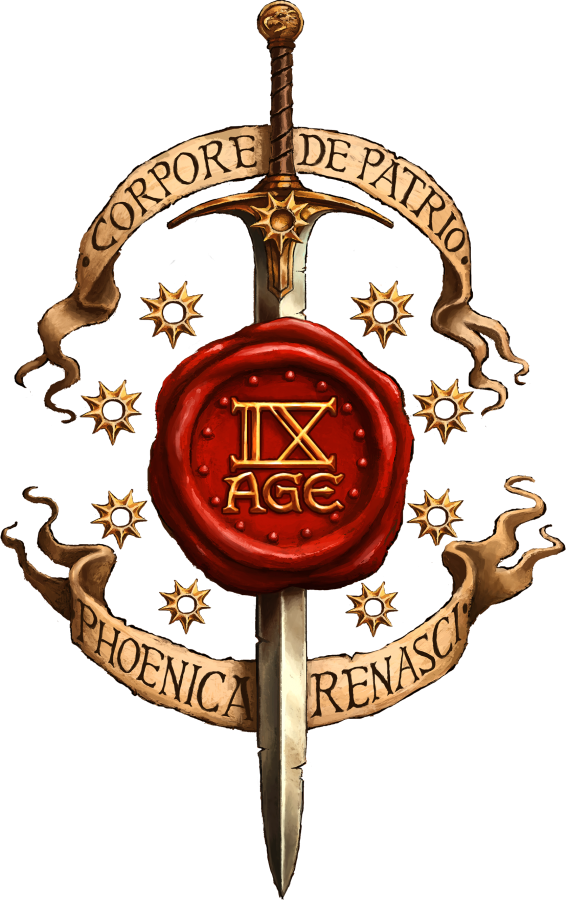
\includegraphics[width=9cm]{../Layout/pics/logo_9th.png}
\vfill
{\antiquefont\fontsize{12}{14.4}\selectfont \textit{\labels@creators}} \\


\end{center}

\newpage

\thispagestyle{empty}

\vphantom{1pt}
\vfill

{\fontsize{12}{14.4}\selectfont

\labels@secondpageannouncement{}

\noindent\newrule{\labels@rulechanges}

\bigskip
\noindent \labels@latexcredit
}


\end{titlepage}

\restoregeometry

\armyspecialrules

\armyspecialruleentry{\masterofundeath}

\newrule{Only models with this special rule can be chosen as General. The General is automatically designated as Master and must exchange one spell for \necromancysignaturespell{}, regardless of which Path it uses.}

\newrule{At the start of any of your player turns in which the army does not have a living Master you must nominate a character with this special rule and knowledge of at least one spell from the Path of \necromancy{}. If that character passes a Leadership test it immediately becomes the new Master.}

\armyspecialruleentry{\ashestoashes}

\newrule{At the end of the phase in which the General is killed, and each time a Leadership test is failed for gaining a new Master (or if there is no eligible character to take the test), all units with the majority of the models having this special rule must take a Leadership Test. If failed the unit suffers 1 wound for each point by which the test was failed with. These wounds are distributed following the rules for \unstable{} but can never be assigned to models without this special rule.}

\armyspecialruleentry{\newrule{\chillingshriek{X, Y}}}

Part of a model with this special rule may perform a shooting \newrule{special} attack with \range{8}. It can be used after marching and hits automatically. The target suffers X hits with strength equal to Y plus the current number of Wounds of the shooting part of model, where X and Y are the number within the brackets. When rolling to wound, compare the Strength with the target's Leadership instead of Toughness. Wounds caused are \armourpiercing{6} and \magicalattacks{}. In the combat phase the model may replace its normal attacks to instead scream at one unit that it is in base contact with it.

\armyspecialruleentry{\awaken{X}}

Models with this special rule can \raisewounds{} of all the units stated within the brackets above their starting size, using any effect with \raisewounds{}. A unit's starting size is the size they are written as in the army list. Units can be increased even beyond the maximum size written in their unit entry using this rule.

\armyspecialruleentry{\invocation{X}}

Models with this special rule can heal wounds back with \necromancysignaturespell{} equal to the amount stated in brackets. A unit cannot be increased above its starting size unless affected by a caster with the \awaken{} special rule.

\armyspecialruleentry{\reaper}

\newrule{Units consisting solely of models with this special rule may move through \removedrule{enemy} units during the Remaining Moves Sub-Phase. All Models in such units can make a single close combat attack against a single unengaged enemy unit which has been moved through. These attacks hit automatically and are distributed towards the unit as a whole.}

\armyspecialruleentry{\vampiric{X}}

Models with this special rule can make march moves as normal even when outside the range of the General's \inspiringpresence{}. They still have to test Leadership if they are within \distance{8} of enemy units. 

\newrule{At the end of the close combat phase, units with this special rule can make a single \vampiric{} roll if a model part with this special rule caused at least one wound during the phase. Roll a D6 for each \vampiric{} roll. On the roll of X+ a single wound is Raised to the unit, where X is the number stated within the brackets (a \result{1} is always a failure). Characters must cause wounds and roll for Raised wounds separately from any unit they are joined to.}

\armyspecialruleentry{\wakethedead}

Each time after an Augment spell from Path of \necromancy{} (including the \necromancyattribute{}) is resolved against a unit containing at least one model with this rule, you may select a single unit within \distance{6} of it. Until the end of the following player turn, all models in the chosen units have the \lightningreflexes{} special rule.

\armyspecialruleentry{\necromanticaura}

\newrule{Units with this special rule and friendly units within range reduce the number of wounds caused by the \ashestoashes{} and \unstable{} special rules by 1. Units with this special rule has a range equal to \distance{6}. The Battle Standard Bearer automatically has this special rule but with the range of its \holdyourground{} instead.}


\armynewsection{\bloodlines}

\vampirelords{} and \vampireheroes{} may purchase unique upgrades called \bloodpowers{}, separated in two categories called \bloodlinepowers{} and \ancientbloodpowers{}. Vampires may also be upgraded to become part of a \bloodline{}, granting them additional bonuses and sometimes restrictions. The \vampirelords{} and \vampireheroes{} of an army must either belong to the same \bloodline{} or none at all.

\armynewsubsection{\bloodline{} Vampires}

May only purchase powers that are specific to that \bloodline{}. \bloodlinepowers{} may be picked by any
Vampire and \ancientbloodpowers{} may only be taken by \vampirelords{}. \bloodlinepowers{} can be duplicated, \ancientbloodpowers{} are \oneofakind{}.

\armynewsubsection{Independent Vampires}

A Vampire that is not part of a \bloodline{} may choose between non \ancientbloodpowers{} of all the \bloodlines{}. All \bloodlinepowers{} are \oneofakind{}.

\armynewsubsection{\bloodties{X}}

Certain unit entries in this army book bear the mention \bloodties{}, followed by the name of a \bloodline{} between brackets. If the \bloodline{} of the Vampire characters in the army matches the one written within the brackets, you gain access to the upgrade written in this rule on the unit entry.

\separator

\armynewsubsection{\brotherhood{} \bloodline\dotfill \pts{35/25}}

A \brotherhood{} Vampire gains +2 Weapon Skill and wears \platearmour{}. He is restricted to purchasing
only one additional Magic Level and may only use Path of \necromancy{}. A \brotherhood{} Vampire cannot
refuse challenges and must issue one whenever possible, unless another Vampire from the same \bloodline{} does it first.

\bloodties{}: \vampireknights{}.

\startpricelist

\pricelistitem{Crimson Rage}{65} \textbf{\ancientbloodpower}. For each unsaved wound the Vampire causes in close combat, it immediately makes another close combat attack. These additional attacks cannot confer more attacks.

\pricelistitem{\newrule{Perfect Warrior}}{35} \textbf{\bloodlinepower}. The Vampire has the \weaponmaster{} and \lethalstrike{} special rules. It is equipped with an \ahw , a \halberd , a \gw , a \lance{} and a \shield{}.

\pricelistitem{\newrule{Eternal Duellist}}{30} \textbf{\bloodlinepower}. The Vampire may re-roll to hit and to
wound rolls in challenges.

\endpricelist

\separator

\armynewsubsection{\strigoi{} \bloodline\dotfill \pts{50/40}}

The Vampire's model has +1 Wound, \regeneration{\newrule{5}} and \hatred{}. The Vampire cannot select any mount except for the \shriekinghorror{}, may not wear any kind of Armour, can only purchase a single additional Magic Level and must use Path of \wilderness{} or \necromancy{}.

\bloodties{}: \ghouls{}.

\startpricelist

\pricelistitem{\newrule{Ghoul Lord}}{65} \textbf{\ancientbloodpower}. The Vampire gains the special rules \poisonedattacks and \armourpiercing{1}. All \ghouls{} in the same unit as the Vampire have \hatred{} and
\armourpiercing{1}.

\pricelistitem{Curse of the Blood}{70} \textbf{\bloodlinepower}. The Vampire gains the special rule
\regeneration{5}. If the Vampire already has \regeneration{} then its save is increased by \newrule{1} point to a maximum of 4+. All \ghouls{} in the same unit as the Vampire, and any mount ridden by the Vampire, gains the special rules \regeneration{6}. If they already have \regeneration{} then their save is increased by 1 point to a maximum of 4+.

\pricelistitem{\newrule{Bat Form}}{\newrule{65/40}} \textbf{\bloodlinepower}. The Vampire gains the special rules \thunderouscharge{} and \fly{8}.

\endpricelist

\separator

\armynewsubsection{\vonkarnstein{} \bloodline\dotfill \pts{25/20}}

The presence of one or more \vonkarnstein{} Vampires grants +1 Combat Score. Undead units joined by the Vampire may march as if they had the \vampiric{} special rule. The range of \inspiringpresence{} and \holdyourground{} of the Vampire is increased by \distance{6}. In addition, the Vampire may re-roll failed \vampiric{} rolls.

\bloodties{}: \darkcoach .

\startpricelist

\pricelistitem{\newrule{Storm Caller}}{50} \textbf{\ancientbloodpower}. All units within \distance{12} of the Vampire gains the \blurry{} special rule. Once per game the Vampire can grant \lightningattacks{} and \armourpiercing{2} to itself and all models part of the same unit. This ability is activated at the start of a combat round and lasts until the end of the player turn.

\pricelistitem{Refined Taste}{25} \textbf{\bloodlinepower}. The Vampire has the \vampiric{2} special rule. \newrule{If mounted on a \largetarget{} it instead has \vampiric{4}}.

\pricelistitem{\newrule{Hour of the Wolf}}{20} \textbf{\bloodlinepower}. The Vampire gains the \awaken{\zombies , \direwolves , \batswarms , \greatbats} special rule. The Vampire gains \swiftstride{} and confers this special rule to any unit it joins.

\endpricelist

\separator

\armynewsubsection{\lamia{} \bloodline\dotfill \pts{35/25}}

The Vampire has +2 Ballistic Skill, -1 Attack, \lightningreflexes{} and \throwingweapons{}. If the Vampire is not wearing any Armour it also has the \distracting{} special rule.

\bloodties{}: \courtofthedamned .

\startpricelist

\pricelistitem{Commandment}{50} \textbf{\ancientbloodpower}. All Rank and File models in any unit joined by the Vampire have Weapon Skill 5. If the Vampire is not engaged in combat itself, it can instead choose to grant this bonus to a single friendly unit within \distance{6}.

\pricelistitem{\newrule{Mask of Innocence}}{25} \textbf{\bloodlinepower}. Enemy units in base contact with one or more Vampire with this power have -1 Leadership.

\pricelistitem{\newrule{Mesmerizing Gaze}}{25} \textbf{\bloodlinepower}. Units charging at or fleeing from units containing at least one Vampire with this power roll an additional dice for their charge or flee move and discard the highest.

\endpricelist

\separator

\armynewsubsection{\nosferatu{} \bloodline\dotfill \pts{\newrule{140/70}}}

The Vampire is a Level 4/2 \wizard{}, has -1 Attack, -2 Weapon Skill, cannot take any kind of Armour, generates an additional spell and has the \awaken{\zombies , \skeletons} special rule.

A \nosferatu Vampire may generate spells from more than one Path of Magic. Which Paths and how many spells from each Path will be generated has to be stated on the army list.

\bloodties{}: \wraiths .

\startpricelist

\pricelistitem{\newrule{Unbearable Scrutiny}}{50} \textbf{\ancientbloodpower}. At the start of each Magic Phase, the Player may nominate an enemy \wizard{} within \distance{18} of the Vampire and within Line of Sight. That \wizard{} cannot add his Magic Level or use \aideddispel{} against spells cast by this Vampire during this phase.

\pricelistitem{\newrule{Arcane Knowledge}}{25} \textbf{\bloodlinepower}. Non-vortex spells cast by the Vampire gain an additional \distance{3} range. Damage spells instead gain an additional \distance{6}.

\pricelistitem{Forbidden Path}{20} \textbf{\bloodlinepower}. Select a Battle Magic Path other than Path of \nature . The Vampire can generate spells from this Path in addition to those normally available to it.

\endpricelist

\armymagicitems

\armymagicweapons

\startpricelist

\pricelistitem{\newrule{Bow of Nepharet}}{45} This is a \boltthrower{} \artilleryweapon{} with the following profile: \range{36}, Strength 6, \armourpiercing{1}, \multiplewounds{D3}{}.

\pricelistitem{Blade of Red Thirst}{40} \newrule{Vampires only}. Type: \hw . \newrule{The model gains \vampiric{5} if mounted on a \largetarget{} and \vampiric{3} otherwise}. The Model part makes a \vampiric{} roll for each \newrule{unsaved} wound cause by this weapon instead of just one. Any excess wounds Raised can be used to \raisewounds{} on the unit that the model is part of.

\endpricelist

\armymagicarmor

\startpricelist

\pricelistitem{\newrule{Red Plate of Gilles de Raux}}{\newrule{40}} Type : \platearmour . Wearer has +1 Wound.

\endpricelist

\armytalismans

\startpricelist

\pricelistitem{\newrule{Mantle of Night}}{40} \newrule{Models on foot only}. Enemy models in base contact with wearer, and all models allocating close combat attacks at the wearer, do not gain strength bonuses \newrule{of the +X type} conferred by mundane or magical weapons.

\endpricelist

\armyenchanteditems

\startpricelist

\pricelistitem{\newrule{Tullius' Teeth}}{\newrule{50}} \removedrule{Models on foot only}. Wearer and other \rnf{} models in its unit have the \distracting{} special rule.

\endpricelist

\armyarcaneitems

\startpricelist

\pricelistitem{Unholy Tome}{35} \boundspell{4}. Contains the spell \necromancyspelltwo{} from Path of \necromancy .

\pricelistitem{\newrule{Staff of the Vengeful Dead}}{35} \boundspell{3}. If cast successfully this item
casts an Augment, Lasts one turn spell with range \distance{6}. All \undead{} models in target unit gain +1 Attack.

\pricelistitem{\newrule{Eye of Setesh}}{20} At the end of any Magic Phase, the play may save one unused Magic Dice and add it to the pool of Magic Dice in the next Magic Phase (immediately after rolling Winds of Magic).

\endpricelist

\armymagicbanners

\startpricelist

\pricelistitem{\newrule{Black Standard of Zagvozd}}{75} The unit carrying this banner has \bodyguard{\vampirelord , \vampirehero}. \vampireknights{} carrying this banner have the \stubborn{} special rule instead. All models in the unit carrying this banner also have \wardsave{4} against all Ranged Attacks.

\pricelistitem{\newrule{Banner of the Barrows Kings}}{50} \barrowknights , \barrowguards{} and \barrowkings{} in this unit have +1 to Hit in close combat.

\endpricelist




%%%%%%%%%%%%%%%%%%%%%%%%%%%%%%%%%%%%%%%%%%%%%%%%%%%%%%%%%%%%%%%%%%%%%%%%%%%%%%%%%%%%%%%%%%%%%%%%%
%%%%%																						%%%%%
%%%%% TRANSLATORS SHOULDN'T HAVE TO EDIT THE CODE PAST THIS LINE - TRANSLATION IS AUTOMATED %%%%%
%%%%%					(unless you want to edit the changelog)								%%%%%
%%%%%%%%%%%%%%%%%%%%%%%%%%%%%%%%%%%%%%%%%%%%%%%%%%%%%%%%%%%%%%%%%%%%%%%%%%%%%%%%%%%%%%%%%%%%%%%%%



\armylist

\lordstitle

\showunit{
	name={\vampirelord},
	cost={200},
	profile={ < 6 7 5 5 5 3 7 5 10},
	type=\infantry ,
	basesize=20x20,
	unitsize=1,
	commontype=\vampiriccommonrules ,
	commonspecialrules={\undead,\fear,\vampiric{6}},
	specialrules={\awaken{\zombies},\masterofundeath},
	magiclevel=1,
	magicpaths={\necromancy, \shadows, \death},
	options={
		\bloodlinechoice = \unlimited,
		\bloodpowerchoice = \unlimited,
		\magicitemsallowance = \upto < 100,
		\magiclevelchoice{
			\magiclevel{2}=30,
			\magiclevel{3}=75,
		},
		\anyofthefollowing{
			\la =5,
			\ha =10,
			\shield =5,
		},
		\weapononechoice{
			\ahw =5,
			\halberd =10,
			\gw =15,
			\lance =\newrule{20},
		}
	},
	mounts={\skeletalsteed =20, \monstrousrevenant =100, \courtofthedamned{} \only{\lamia}=190, \shriekinghorror{} \only{\strigoi}=200, \zombiedragon =280}
}

\showunit{
	name={\necromancerlord},
	cost={150},
	profile={ < 4 3 3 3 4 3 3 1 8},
	type= \infantry ,
	basesize=20x20,
	unitsize=1,
	commontype=\undeadcommonrules ,
	commonspecialrules={\undead},
	specialrules={\awaken{\zombies , \skeletons}, \masterofundeath},
	magiclevel=3,
	magicpaths={\necromancy, \fire, \death},
	options={
		\magicitemsallowance = \upto < 100,
		\magiclevel{4}=60,
	},
	mounts={\skeletalsteed =20, \monstrousrevenant =100, \cadaverwagon =100}
}

\heroestitle


\showunit {
	name={\vampirehero},
	cost=80,
	profile={ < 6 6 4 5 4 2 6 4 8},
	type=\infantry ,
	basesize=20x20,
	unitsize=1,
	commontype=\vampiriccommonrules ,
	commonspecialrules={\undead,\fear,\vampiric{6}},
	specialrules={\awaken{\zombies}, \masterofundeath},
	magicpaths={\necromancy, \shadows, \death},
	options={
		\bloodlinechoice =\unlimited,
		\bloodpowerchoice =\unlimited,		
		\magicitemsallowance = \upto < 50,
		\bsboption{} \notif{\strigoi}= 25,
		\magiclevelchoice{
			\magiclevel{1}=25,
			\magiclevel{2}=55,
		},
		\anyofthefollowing{
			\la =5,
			\ha =10,
			\shield =5,
		},
		\weapononechoice{
			\ahw =5,
			\halberd =5,
			\gw =10,
			\lance =\newrule{15},
		}
	},
	mounts={\skeletalsteed =20, \monstrousrevenant =120}
}


\showunit{
	name={\necromancer},
	cost={60},
	profile={ < 4 3 3 3 3 2 3 1 7},
	type= \infantry ,
	basesize=20x20,
	unitsize=1,
	commontype=\undeadcommonrules ,
	commonspecialrules={\undead},
	specialrules={\awaken{\zombies, \skeletons}, \masterofundeath},
	magiclevel=1,
	magicpaths={\necromancy, \fire, \death},
	options={
		\magicitemsallowance = \upto < 50,
		\magiclevel{2}=30,
	},
	mounts={\skeletalsteed = \newrule{20}, \cadaverwagon = 100}
}

\showunit{
	name={\barrowking},
	cost=80,
	profile={ < 4 4 - 4 5 3 4 3 9},
	type=\infantry ,
	basesize=20x20,
	unitsize=1,
	commontype=\undeadcommonrules ,
	commonspecialrules={\undead},
	specialrules={\multiplewounds{2}{\infantry, \cavalry, \warbeasts}, \lethalstrike, \notaleader, \newrule{\magicalattacks}},
	equipment={\ha, \shield},
	options={
		\magicitemsallowance = \upto < 50,
		\bsboption = 25,
		\weapononechoice{
			\ahw =5,
			\halberd =5,
			\lance =5,
			\gw =10,
		},
		\maybeupgradedto{} \unlivingshield = 15
	},
	mounts={\skeletalsteed = \newrule{20}},
	unitrules={
		\unitrule{\unlivingshield}{\unlivingshieldrule}
	}
}

\showunit {
	name={\fellwraith},
	cost=65,
	profile={\fellwraith < 6 3 - 3 3 2 2 \newrule{3} 5,
		     \banshee 	 < 6 3 - 3 3 2 3 \newrule{1} 5
	},
	type=\infantry ,
	basesize=20x20,
	unitsize=1,
	commontype=\undeadcommonrules ,
	commonspecialrules={\undead, \ashestoashes},
	specialrules={\ethereal, \reaper, \notaleader, \terror},
	options={
		\mustbecomeoneofthefollowing{
			\fellwraith = \free,
			\banshee = 30
		}
	},
	additional={%
		\separator
		\begin{multicols}{2}
		\begin{center} \LARGE\antiquefont\fellwraith \end{center}
		
		{\setlength{\parskip}{0.1cm}
			\noindent\textbf{\labels@specialrules :}\expandafter\ruleslist\expandafter{%
				\armourpiercing{6}%
			}.
		
			\noindent\textbf{\labels@equipment :}\expandafter\equipmentlist\expandafter{%
				\gw%
			}.
		}

		\vspace*{0.15cm}\mountsframestart\expandafter\mountslist\expandafter{%
			\newrule{\skeletalsteed} = \newrule{20}%
		}\mountsframeend
			
		\columnbreak
		\begin{center} \LARGE\antiquefont\banshee \end{center}
		
		\noindent\textbf{\labels@specialrules :}\expandafter\ruleslist\expandafter{%
			\chillingshriek{2, 8}%
		}.
		\end{multicols}
	},
}


\coreunitstitle

\showunit{
	name={\zombies},
	cost=60,
	profile={ < 4 1 0 3 3 1 1 1 2},
	invocation={2D6+3},
	type=\infantry ,
	basesize=20x20,
	unitsize=20,
	additionalmodels=40,
	costpermodel=3,
	commontype=\undeadcommonrules ,
	commonspecialrules={\undead, \ashestoashes},
	commandgroup={musician=10, banner=10}
}

\showunit{
	name={\skeletons},
	cost=40,
	profile={< 4 2 2 3 3 1 2 1 6},
	invocation={1D6+3},
	type=\infantry ,
	basesize=20x20,
	unitsize=10,
	additionalmodels=50,
	costpermodel=4,
	commontype=\undeadcommonrules ,
	commonspecialrules={\undead, \ashestoashes},
	equipment={\la},
	options={
		\spear = \free,
		\shield = \permodel < 1
	},
	commandgroup={champion=10, musician=10, banner=10, veteranbannerallowance=\newrule{25}}
}

\showunit{
	name={\ghouls},
	cost=90,
	profile={< 4 3 - 3 4 1 3 2 6},
	invocation={1D6+3},
	type= \infantry ,
	basesize=20x20,
	unitsize=10,
	additionalmodels=30,
	costpermodel=9,
	commontype=\undeadcommonrules ,
	commonspecialrules={\undead, \ashestoashes},
	specialrules={\poisonedattacks},
	options={
		\skirmishers{} \ifNmodelsorless{15}= \permodel < 1,
		\bloodties{\strigoi}:\newline\vanguard{}*= \permodel < 2,
	},
	commandgroup={champion=10, musician=10, bannerrestriction=\unitwith{} \vanguard , banner=10, musicianrestriction=\unitwith{} \vanguard , veteranbannerallowance = \newrule{25}},
	additional={%
		\vspace*{0.1cm}		
		* \strigoivanguardnote
	}
}

\showunit{
	name={\direwolves},
	cost=40,
	profile={
		< 9 3 0 3 3 1 3 1 3},
	invocation={1D3+3},
	type=\warbeast ,
	basesize=25x50,
	unitsize=5,
	additionalmodels=10,
	costpermodel=7,
	commontype=\undeadcommonrules ,
	commonspecialrules={\undead, \ashestoashes},
	specialrules={\vanguard, \thunderouscharge},
	commandgroup={champion=10}
}

\showunit{
	name={\batswarm},
	cost=60,
	profile={
		< 1 2 - 2 2 4 3 4 3},
	invocation={1D6+3},
	type=\swarm ,
	basesize=40x40,
	unitsize=2,
	additionalmodels=8,
	costpermodel=15,
	commontype=\undeadcommonrules ,
	commonspecialrules={\undead, \ashestoashes},
	specialrules={\fly{6}},
	unitrules={
		\unitrule{\stormofwings}{\stormofwingsrule}
	}
}

\specialunitstitle


\showunit{
	name={\barrowknights},
	cost=120,
	profile={\knight < 4 3 - 4 4 1 3 1 6,
			  \steed < 8 2 - 3 3 1 2 1 3
	},
	invocation= 2 ,
	type=\cavalry ,
	basesize=25x50,
	unitsize=5,
	additionalmodels=10,
	costpermodel=24,
	commontype=\undeadcommonrules ,
	commonspecialrules={\undead, \ashestoashes},
	specialrules={\magicalattacks, \multiplewounds{2}{\infantry , \cavalry , \warbeasts}, \lethalstrike{} \only{\knight}, \ethereal{} \only{\steed}},
	equipment={\ha , \shield , \lance , \mountsprotection{5}},
	commandgroup={champion=10, musician=10, banner=10, bannerallowance=50}
}

\showunit{
	name={\barrowguards},
	cost=100,
	profile={
		< 4 3 - 4 4 1 3 1 8},
	invocation= 1D3+3 ,
	type=\infantry,
	basesize=20x20,
	unitsize=10,
	additionalmodels=30,
	costpermodel=10,
	commontype=\undeadcommonrules ,
	commonspecialrules={\undead, \ashestoashes},
	specialrules={\magicalattacks, \multiplewounds{2}{\infantry , \cavalry , \warbeasts},\lethalstrike, \bodyguard{\general, \barrowking}},
	equipment={\ha},
	options={
		\shield = \permodel < 1,
		\weapononechoice{
			\halberd = \permodel < 2,
			\gw = \permodel < 2
		},
	},
	commandgroup={champion=10, musician=10, banner=10, bannerallowance=50}
}

\showunit{
	name={\ghasts},
	cost=110,
	profile={< 6 3 - 4 5 3 2 3 5},
	invocation= 2 ,
	type=\monstrousinfantry ,
	basesize=40x40,
	unitsize=3,
	additionalmodels=7,
	costpermodel=48,
	commontype=\undeadcommonrules ,
	commonspecialrules={\undead, \ashestoashes},
	specialrules={\poisonedattacks, \fear,  \regeneration{5}},
	commandgroup={champion=10}
}

\showunit{
	name={\vampirespawn},
	cost=126,
	profile={
		< 6 4 - 5 4 3 4 3 8},
	invocation= 2 ,
	type=\monstrousinfantry ,
	basesize=40x40,
	unitsize=3,
	additionalmodels=5,
	costpermodel=42,
	commontype=\vampiriccommonrules ,
	commonspecialrules={\undead, \vampiric{6}, \fear},
	specialrules={\frenzy, \skirmishers, \fly{9}},
	commandgroup={champion=10}
}

\showunit{
	name={\phantomhost},
	cost=70,
	profile={< 6 3 - 3 3 4 1 4 4},
	invocation= 1D3+3 ,
	type=\infantry,
	basesize=40x40,
	unitsize=2,
	additionalmodels=4,
	costpermodel=35,
	commontype=\undeadcommonrules ,
	commonspecialrules={\undead, \ashestoashes},
	specialrules={\ethereal, \fear}
}

\showunit{
	name={\greatbats},
	cost=40,
	profile={
		< 1 3 - 3 3 2 3 2 3},
	invocation= 1D3+3 ,
	type=\warbeast ,
	basesize=40x40,
	unitsize=2,
	additionalmodels=7,
	costpermodel=14,
	commontype=\undeadcommonrules ,
	commonspecialrules={\undead, \ashestoashes},
	specialrules={\skirmishers, \fly{10}},
}

\showunit{
	name={\varkolak},
	cost=\newrule{165},
	profile={
		< 8 5 - 6 5 4 4 5 7},
	invocation= 1 ,
	type=\monstrousbeast ,
	basesize=50x50,
	unitsize=1,
	commontype=\vampiriccommonrules ,
	commonspecialrules={\undead, \vampiric{3}, \fear},
	specialrules={\hatred, \regeneration{4}},
	options={
		\maytakeoneofthefollowing{
			\vanguard{}= 20,
			\stomp{1D3+1}= 20,
			\fly{8}= 40,
		}
	}
}

\showunit{
	name={\cadaverwagon},
	cost=80,
	profile={
		\cadaverwagon < - - - 4 4 4 - - -,
   		\cadavermaster < - 3 - 3 - -  3 1 5,
		\shamblinghorde < 4 1 - 3 3 -  1 * -	
	},
	invocation= 1 ,
	type=\chariot ,
	basesize=50x100,
	unitsize=1,
	commontype=\undeadcommonrules ,
	commonspecialrules={\undead, \ashestoashes},
	specialrules={\randomattacks{2D6} \only{\shamblinghorde}, \wakethedead, \cart, \regeneration{4}},
	equipment={\mountsprotection{5}},
	options={
		\endlesshorde = 25,
		\maytakeoneofthefollowing{
			\bonepyre = 10,
			\bringoutyourdead = 15,
			\necromanticaura = 20
		}
	},
	unitrules={
		\unitrule{\cart}{\cartrule}
		\unitrule{\endlesshorde}{\endlesshorderule}
		\unitrule{\bonepyre}{\bonepyrerule}
		\unitrule{\bringoutyourdead}{\bringoutyourdeadrule}
	}
}

\rareunitstitle


\showunit{
	name={\vampireknights},
	cost=225,
	profile={
		\knight < 4 5 3 5 4 2 5 2 8,
		\undeadmount < 8 3 0 4 3 1 2 1 3
	},
	invocation= 2 ,
	type=\cavalry ,
	basesize=25x50,
	unitsize=5,
	additionalmodels=5,
	costpermodel=45,
	commontype=\vampiriccommonrules ,
	commonspecialrules={\undead,\fear,\vampiric{6}},
	equipment={\lance , \ha , \shield , \mountsprotection{6}, \barding},
	options={
		\bloodties{\brotherhood}:\newline\platearmour{} \wordand{} \devastatingcharge{}= \permodel < 15
	},
	commandgroup={champion=10, musician=10, banner=10, bannerallowance=75}
}

\showunit{
	name={\wraiths},
	cost=\newrule{150},
	profile={
		< 6 3 - 3 3 2 2 2 5
	},
	invocation= 2,
	type=\infantry,
	basesize=20x20,
	unitsize=5,
	additionalmodels=\newrule{3},
	costpermodel=\newrule{30},
	commontype=\undeadcommonrules ,
	commonspecialrules={\undead, \ashestoashes},
	specialrules={\wizardconclave{\Level{} \newrule{2}, \deathsignaturespell{} (Path of \death), \newrule{\shadowssignaturespell{} (Path of \shadows)}}, \ethereal,  \bodyguard{\fellwraith , \banshee}, \reaper, \armourpiercing{6}, \terror, \skirmishers},
	equipment={\gw},
	commandgroup={champion=70, championprerestriction=\bloodties{\nosferatu}:},
}

\showunit{
	name={\mountedwraiths},
	cost=150,
	profile={\rider < 6 3 - 3 3 1 2 1 5,
	         \steed < 8 2 - 3 3 1 2 1 3
	},
	invocation= 2,
	type=\cavalry ,
	basesize=25x50,
	unitsize=5,
	additionalmodels=5,
	costpermodel=30,
	commontype=\undeadcommonrules ,
	commonspecialrules={\undead, \ashestoashes},
	specialrules={\flamingattacks{} \only{\rider}, \ethereal, \reaper, \armourpiercing{6} \only{\rider}, \freereform, \terror},
	equipment={\gw , \mountsprotection{6}},
	commandgroup={champion=10}
}

\showunit{
	name={\wingedreapers},
	cost=150,
	profile={
        	< 6 5 3 5 5 4 4 3 10,
	},
	invocation= 2,
	type=\monstrousinfantry ,
	basesize=50x75,
	unitsize=2,
	additionalmodels=3,
	costpermodel=75,
	commontype=\undeadcommonrules ,
	commonspecialrules={\undead, \ashestoashes},
	specialrules={\necromanticaura, \undeadconstructs, \lethalstrike, \terror, \fly{6}},
	equipment={\innatedefence{5}},
	options={
			\la = \permodel < 10,
		\weapononechoice{
			\ahw = \permodel < 5,
			\halberd = \permodel < 10
		}
	},
	unitrules={
		\unitrule{\undeadconstructs}{\undeadconstructsrule}
	},
}

\showunit{
	name={\altarofundeath},
	cost=200,
	profile={
		\altarofundeath < -  - - 5 5 5 - - -,
       	\master{} (1) < -  3 1 3 - - 3 1 5,
		\banshee{} (0)[1] < -  3 - 3 - [2] 3 3 5,
		\ghoststeeds{} (1) < 8 3 - 3 - - 2 * 4
	},
	invocation= 1,
	type=\chariot ,
	basesize=50x100,
	unitsize=1,
	commontype=\undeadcommonrules ,
	commonspecialrules={\undead, \ashestoashes},
	specialrules={\randomattacks{2D6} \only{\ghoststeeds}, \auraofundeath, \chillingshriek{2,8} \only{\banshee},  \ethereal{} \only{\ghoststeeds}, \largetarget , \terror , \regeneration{4}},
	equipment={\innatedefence{5}},
	options={
		\maytakeoneofthefollowing{
			\banshee{} (1)= 20,
			\darktome = 20
		}
	},
	unitrules={
		\unitrule{\darktome}{\darktomerule}
		\unitrule{\auraofundeath}{\auraofundeathrule}
	}
}

\showunit{
	name={\shriekinghorror},
	cost=200,
	profile={
        	< 6 4 - 5 6 6 2 4 4,
	},
	invocation= 1,
	type=\monster ,
	basesize=100x150,
	unitsize=1,
	commontype=\undeadcommonrules ,
	commonspecialrules={\undead, \ashestoashes},
	specialrules={\chillingshriek{6, 4}, \regeneration{6}, \fly{8}},
}

\showunit{
	name={\darkcoach},
	cost=190,
	profile={
		\darkcoach 				< - - - 5 6 4 - - -,
        \fellwraith{} (1) 		< - 3 - 3 - - 3 3 5,
		\awakenedvampire{} (*) 	< - 6 - 5 - - 6 4 8,
		\undeadmount{} (2) 		< 8 3 - 4 - - 2 1 -
	},
	invocation= 1,
	type=\chariot ,
	basesize=50x100,
	unitsize=1,
	commontype=\vampiriccommonrules ,
	commonspecialrules={\undead , \vampiric{4}},
	specialrules={\soulsyphon, \scythes, \wardsave{4}, \terror},
	equipment={\ha, \mountsprotection{5}, \gw{} \only{\fellwraith}},
	options={
		\bloodties{\vonkarnstein}:\newline\stubborn = 30
	},
	unitrules={
		\unitrule{\soulsyphon}{\soulsyphonrule}
	},
	additional={\soulsyphonchart},
}

\showunit{
	name={\courtofthedamned},
	cost=190,
	profile={
		\courtofthedamned 	< - - - 5 5 5 - - -,
       	\paramours{} (3) 	< - 5 5 5 - - 6 2 7,
		\ghoststeeds{} (1) 	< 8 3 - 3 - - 2 * 4
	},
	invocation= 1,
	type=\chariot ,
	basesize=50x100,
	unitsize=1,
	commontype=\vampiriccommonrules ,
	commonspecialrules={\undead , \vampiric{6}},
	specialrules={\randomattacks{2D6} \only{\ghoststeeds}, \ethereal{} \only{\ghoststeeds}, \largetarget, \wardsave{4}, \terror},
	equipment={\throwingweapons{} \only{\paramours}, \innatedefence{5}},
	options={
		\bloodties{\lamia}:\newline\wakethedead = 25
	}
}


\mountstitle

\mountssectionannouncement

\showunit{
	name={\skeletalsteed},
	cost={-},
	profile={
        		 < 8 2 - 3 3 1 2 1 3,
	},
	type=\warbeast ,
	basesize=25x50,
	unitsize=1,
	commontype=\undeadcommonrules ,
	commonspecialrules={\undead},
	specialrules={\ethereal{} \only{\steed}},
	equipment={\mountsprotection{6}},
	options={
		\maytakeoneofthefollowing{
			\mountsprotection{5}= \newrule{15},
			\fly{8} \newrule{\onlyasvampiresmount}= \newrule{35}
		}
	}
}

\showunit{
	name={\monstrousrevenant},
	cost={-},
	profile={
		< 6  4 - 5 5 4 2 4 4,
	},
	type=\monstrousbeast ,
	basesize=50x50,
	unitsize=1,
	commontype=\undeadcommonrules ,
	commonspecialrules={\undead},
	specialrules={\largetarget, \fear},
	options={%
		\maytakeuptotwoofthefollowing{
			\poisonedattacks = 5,
			\lethalstrike = 10,
			\vampiric{5}= 15,
			\randomattacks{D6+2}= 30,
			\fly{8}= 40
		},
	}
}


\showunit{
	name={\shriekinghorror},
	cost={-},
	profile={
        	< 6 4 - 5 6 6 2 4 4,
	},
	type=Monstre,
	basesize=100x150,
	unitsize=1,
	commontype=\undeadcommonrules ,
	commonspecialrules={\undead},
	specialrules={\chillingshriek{6,4}, \regeneration{6}, \fly{8}},
}

\showunit{
	name={\cadaverwagon},
	cost=80,
	profile={
		\cadaverwagon < - - - 4 4 4 - - -,
		\shamblinghorde < 4 1 - 3 3 -  1 * -	
	},
	type=\chariot ,
	basesize=50x100,
	unitsize=1,
	commontype=\undeadcommonrules ,
	commonspecialrules={\undead},
	specialrules={\randomattacks{2D6} \only{\shamblinghorde}, \wakethedead, \cart, \regeneration{4}},
	equipment={\mountsprotection{5}},
	options={
		\endlesshorde = 25,
		\maytakeoneofthefollowing{
			\bonepyre = 10,
			\bringoutyourdead = 15,
			\necromanticaura = 20
		}
	},
	unitrules={
		\unitrule{\cart}{\cartrule}
		\unitrule{\endlesshorde}{\endlesshorderule}
		\unitrule{\bonepyre}{\bonepyrerule}
		\unitrule{\bringoutyourdead}{\bringoutyourdeadrule}
	}
}

\showunit{
	name={\courtofthedamned},
	cost=190,
	profile={
		\courtofthedamned 	< - - - 5 5 5 - - -,
       	\paramours{} (2) 	< - 5 5 5 - - 6 2 7,
		\ghoststeeds{} (1) 	< 8 3 - 3 - - 2 * 4
	},
	type=\chariot ,
	basesize=50x100,
	unitsize=1,
	commontype=\vampiriccommonrules ,
	commonspecialrules={\undead , \vampiric{6}},
	specialrules={\randomattacks{2D6} \only{\ghoststeeds}, \ethereal{} \only{\ghoststeeds}, \largetarget, \wardsave{4}, \terror},
	equipment={\throwingweapons{} \only{\paramours}, \innatedefence{5}},
	options={
		\bloodties{\lamia}:\newline\wakethedead = 25
	}
}

\showunit{
	name={\zombiedragon},
	cost={-},
	profile={
		< 6  4 - 6 6 6 2 5 4,
	},
	type=\monster ,
	basesize=50x100,
	unitsize={1},
	commontype=\undeadcommonrules ,
	commonspecialrules={\undead},
	specialrules={\breathweapon{\Strength{} 2, \armourpiercing{6}}, \distracting, \regeneration{6}, \fly{7}},
	equipment={\innatedefence{4}},
	options={
		\maybeupgradedto{} \colossalzombiedragon{}= 40
	},
	unitrules={
		\unitrule{\colossalzombiedragon}{\colossalzombiedragonrule}
	}
}

\quickrefsheettitle

% Script to automatically draw the Quick Ref Sheet

\renewcommand{\arraystretch}{1.2}

\providebool{QRSbool}

\providebool{whiterow}

\newcommand{\QRSrowcolor}{\ifbool{whiterow}{\global\boolfalse{whiterow}}{\rowcolor{black!10}\global\booltrue{whiterow}}}

\newcommand{\QRSstarttab}[1]{%
	\noindent%
	\setlength{\tabcolsep}{2pt}%
	\begin{tabular}{@{}cp{3.2cm}M{\profilecellsize}@{}M{\profilecellsize}@{}M{\profilecellsize}@{}M{\profilecellsize}@{}M{\profilecellsize}@{}M{\profilecellsize}@{}M{\profilecellsize}@{}M{\profilecellsize}@{}M{\profilecellsize}}%

	& \antiquefont\large{\textbf{#1}} & \textbf{\labels@M} & \textbf{\labels@WS} & \textbf{\labels@BS} & \textbf{\labels@S} & \textbf{\labels@T} & \textbf{\labels@W} & \textbf{\labels@I} & \textbf{\labels@A} & \textbf{\labels@Ld}%
}%

\newcommand{\QRSclosetab}{\end{tabular}\bigskip}%

\newcommand{\QRSprintline}[4]{%
	\tabularnewline%
	\ifnumequal{\rowmulti}{1}{\QRSrowcolor}{}%
	\DTLifeq*{\rowcategory}{\labels@lords}{\antiquefont\bfseries \labels@lordsInitial}{}%
	\DTLifeq*{\rowcategory}{\labels@heroes}{\antiquefont\bfseries \labels@heroesInitial}{}%
	\DTLifeq*{\rowcategory}{\labels@coreunits}{\antiquefont\bfseries \labels@coreunitsInitial}{}%
	\DTLifeq*{\rowcategory}{\labels@specialunits}{\antiquefont\bfseries \labels@specialunitsInitial}{}%
	\DTLifeq*{\rowcategory}{\labels@rareunits}{\antiquefont\bfseries \labels@rareunitsInitial}{}%
	\DTLifeq*{\rowcategory}{\labels@mounts}{\antiquefont\bfseries \labels@mountsInitial}{}%
	&%
	\ifnumequal{\rowmulti}{1}{%no Multiprofile
		\rowname%
		\expandafter\parselist\expandafter{\rowprofile}{\locallists@profileslist}%
		\forlistloop{\QRSmonoprofile}{\locallists@profileslist}%
	}{% Multiprofile
		\rowname &&&&&&&&&%
		\expandafter\parselist\expandafter{\rowprofile}{\locallists@profileslist}%
		\forlistloop{\QRSmultiprofile}{\locallists@profileslist}%
	}%
}

\newcommand{\QRSmultiprofile}[1]{%
	\tabularnewline%
	\QRSrowcolor{}&%
	\splitatinf{#1}\local@unitname\local@unitprofile%
	- \local@unitname \expandafter\caraclist\expandafter{\local@unitprofile}%
}%

\newcommand{\QRSmonoprofile}[1]{%
	\splitatinf{#1}\local@unitname\local@unitprofile%
	\expandafter\caraclist\expandafter{\local@unitprofile}%
}%

\newcommand{\QRSprinttab}[1]{%
	\global\booltrue{whiterow}%
	\DTLforeach*[#1]%
	{profiles}{\rowname=name, \rowtrooptype=trooptype, \rowcategory=category, \rowprofile=profile, \rowmulti=multipleprofile}{%
      		\QRSprintline{\rowname}{\rowcategory}{\rowprofile}{\rowmulti}%
	}%
}%

\providebool{QRSisempty}
\global\boolfalse{QRSisempty}%

\newcommand{\QRScheckifempty}[1]{%
	\global\booltrue{QRSisempty}%
	\DTLforeach*[#1]%
	{profiles}{\rowname=name, \rowtrooptype=trooptype, \rowcategory=category, \rowprofile=profile, \rowmulti=multipleprofile}{%
		\global\boolfalse{QRSisempty}\dtlbreak%
	}%
}%

\newcommand{\QRSifnotempty}[1]{%
	\ifbool{QRSisempty}{}{#1}%
}%

\begin{multicols}{2}

\QRScheckifempty{%
	\DTLiseq{\rowcategory}{\labels@lords}\or\DTLiseq{\rowcategory}{\labels@heroes}%
}%
\QRSifnotempty{%
	\QRSstarttab{\characters}%
	\QRSprinttab{%
		\DTLiseq{\rowcategory}{\labels@lords}\or\DTLiseq{\rowcategory}{\labels@heroes}%
	}%
	\QRSclosetab{}%
}%

\QRScheckifempty{%
	\DTLiseq{\rowtrooptype}{\infantry}\and\not\DTLiseq{\rowcategory}{\labels@heroes}\and\not\DTLiseq{\rowcategory}{\labels@lords}%
}%
\QRSifnotempty{%
	\QRSstarttab{\infantry}%
	\QRSprinttab{%
		\DTLiseq{\rowtrooptype}{\infantry}\and\not\DTLiseq{\rowcategory}{\labels@heroes}\and\not\DTLiseq{\rowcategory}{\labels@lords}%
	}% 
	\QRSclosetab{}%
}% 

\QRScheckifempty{%
	\DTLiseq{\rowtrooptype}{\monstrousinfantry}\and\not\DTLiseq{\rowcategory}{\labels@heroes}\and\not\DTLiseq{\rowcategory}{\labels@lords}%
}%
\QRSifnotempty{%
	\QRSstarttab{\monstrousinfantry}%
	\QRSprinttab{%
		\DTLiseq{\rowtrooptype}{\monstrousinfantry}\and\not\DTLiseq{\rowcategory}{\labels@heroes}\and\not\DTLiseq{\rowcategory}{\labels@lords}%
	}% 
	\QRSclosetab{}%
}% 

\QRScheckifempty{%
	\DTLiseq{\rowtrooptype}{\warbeast}\and\not\DTLiseq{\rowcategory}{\labels@heroes}\and\not\DTLiseq{\rowcategory}{\labels@lords}%
}%
\QRSifnotempty{%
	\QRSstarttab{\warbeasts}%
	\QRSprinttab{%
		\DTLiseq{\rowtrooptype}{\warbeast}\and\not\DTLiseq{\rowcategory}{\labels@heroes}\and\not\DTLiseq{\rowcategory}{\labels@lords}%
	}% 
	\QRSclosetab{}%
}% 

\QRScheckifempty{%
	\DTLiseq{\rowtrooptype}{\monstrousbeast}\and\not\DTLiseq{\rowcategory}{\labels@heroes}\and\not\DTLiseq{\rowcategory}{\labels@lords}%
}%
\QRSifnotempty{%
	\QRSstarttab{\monstrousbeasts}%
	\QRSprinttab{%
		\DTLiseq{\rowtrooptype}{\monstrousbeast}\and\not\DTLiseq{\rowcategory}{\labels@heroes}\and\not\DTLiseq{\rowcategory}{\labels@lords}%
	}% 
	\QRSclosetab{}%
}% 

\QRScheckifempty{%
	\DTLiseq{\rowtrooptype}{\cavalry}\and\not\DTLiseq{\rowcategory}{\labels@heroes}\and\not\DTLiseq{\rowcategory}{\labels@lords}%
}%
\QRSifnotempty{%
	\QRSstarttab{\cavalry}%
	\QRSprinttab{%
		\DTLiseq{\rowtrooptype}{\cavalry}\and\not\DTLiseq{\rowcategory}{\labels@heroes}\and\not\DTLiseq{\rowcategory}{\labels@lords}%
	}%
	\QRSclosetab{}%
}% 

\QRScheckifempty{%
	\DTLiseq{\rowtrooptype}{\monstrouscavalry}\and\not\DTLiseq{\rowcategory}{\labels@heroes}\and\not\DTLiseq{\rowcategory}{\labels@lords}%
}%
\QRSifnotempty{%
	\QRSstarttab{\monstrouscavalry}%
	\QRSprinttab{%
		\DTLiseq{\rowtrooptype}{\monstrouscavalry}\and\not\DTLiseq{\rowcategory}{\labels@heroes}\and\not\DTLiseq{\rowcategory}{\labels@lords}%
	}%
	\QRSclosetab{}%
}% 

\QRScheckifempty{%
	\DTLiseq{\rowtrooptype}{\chariot}\and\not\DTLiseq{\rowcategory}{\labels@heroes}\and\not\DTLiseq{\rowcategory}{\labels@lords}%
}%
\QRSifnotempty{%
	\QRSstarttab{\chariots}%
	\QRSprinttab{%
		\DTLiseq{\rowtrooptype}{\chariot}\and\not\DTLiseq{\rowcategory}{\labels@heroes}\and\not\DTLiseq{\rowcategory}{\labels@lords}%
	}%
	\QRSclosetab{}%
}% 

\QRScheckifempty{%
	\DTLiseq{\rowtrooptype}{\monster}\and\not\DTLiseq{\rowcategory}{\labels@heroes}\and\not\DTLiseq{\rowcategory}{\labels@lords}%
}%
\QRSifnotempty{%
	\QRSstarttab{\monsters}%
	\QRSprinttab{%
		\DTLiseq{\rowtrooptype}{\monster}\and\not\DTLiseq{\rowcategory}{\labels@heroes}\and\not\DTLiseq{\rowcategory}{\labels@lords}%
	}%
	\QRSclosetab{}%
}% 

\QRScheckifempty{%
	\DTLiseq{\rowtrooptype}{\swarm}\and\not\DTLiseq{\rowcategory}{\labels@heroes}\and\not\DTLiseq{\rowcategory}{\labels@lords}%
}%
\QRSifnotempty{%
	\QRSstarttab{\swarms}%
	\QRSprinttab{%
		\DTLiseq{\rowtrooptype}{\swarm}\and\not\DTLiseq{\rowcategory}{\labels@heroes}\and\not\DTLiseq{\rowcategory}{\labels@lords}%
	}%
	\QRSclosetab{}%
}% 

\end{multicols}

\changelogtitle

\startchangelog

\newlog{0.10.1}{%
Cleaned up Quick Reference Sheet,
Clarifications added on Von Karnstein, Vampiric, Ashes to Ashes, Blade of Red Thirst and Wake the Dead,
}

\newlog{0.10.0}{%
Leaders of the Undead (reworded),
Nightshroud (clarification),
Wraith Sentries, wizard conclave (typo),
Barrow king special rules (typo),
vampiric and hunger merged into one rule,
Cadaver Wagon, Endless Horde,
Vampire count and baron, lance cost,
Infernal Tome,
Otherworldly Scream, (reworded to a special attack),
Acursed Book, points cost,
Skeletal Steed options costs,
Bat Swarm profile,
Vargbeast Cost,
Ghouls Vanguard allowance to Strigoi Vampire,
Magic Banners for one core,
Strigoi Regen,
Hero Wraith mounting option,
Blade of Red Thirst on Large Targets,
Refined Taste on Large Targets,
Cost on Bloody Hauberk,
Reaper (clarification),
Otherworldly Scream (clarification),
Wraith Sentries, Wizard Conclave
}

\newlog{0.9.3}{%
Skeletons, light armour (missing),
Barrow guard, lethal strike (missing),
Wraith, statline,
}

\newlog{0.9.2}{%
Royal Blood thin power,
Ghoul's invocation value
}

\newlog{0.9.1}{%
Reaper,
Strigoi Bloodline,
Flying Terror points,
Von Castelstein Bloodline,
Nosferatu Bloodline,
The Accursed Book,
Nightshroud,
Skeletons statline,
Ghouls bloodline unit,
Bat Swarm points,
Wraith Sentries,
}

\endchangelog

\end{document}